% !Mode:: "TeX:UTF-8"
\documentclass[12pt,oneside,a4paper]{article}

%%%%%%%%------------------------------------------------------------------------
%%%% 日常所用宏包

%% 控制页边距
% 如果是beamer文档类, 则不用geometry
\makeatletter
\@ifclassloaded{beamer}{}{\usepackage[top=2.5cm, bottom=2.5cm, left=2.5cm, right=2.5cm]{geometry}}
\makeatother

\makeatletter
\@ifclassloaded{beamer}{
\makeatletter
\def\th@mystyle{%
    \normalfont % body font
    \setbeamercolor{block title example}{bg=orange,fg=white}
    \setbeamercolor{block body example}{bg=orange!20,fg=black}
    \def\inserttheoremblockenv{exampleblock}
  }
\makeatother
\theoremstyle{mystyle}
\newtheorem*{remark}{Remark}

\newcommand{\propnumber}{} % initialize
\newtheorem*{prop}{Proposition \propnumber}
\newenvironment{propc}[1]
  {\renewcommand{\propnumber}{#1}%
   \begin{shaded}\begin{prop}}
  {\end{prop}\end{shaded}}

\makeatletter
\newenvironment<>{proofs}[1][\proofname]{%
    \par
    \def\insertproofname{#1\@addpunct{.}}%
    \usebeamertemplate{proof begin}#2}
  {\usebeamertemplate{proof end}}
\makeatother

}{
}
\makeatother
\usepackage{amsthm}

%\DeclareMathOperator{\sech}{sech}
%\DeclareMathOperator{\csch}{csch}
%\DeclareMathOperator{\arcsec}{arcsec}
%\DeclareMathOperator{\arccot}{arccot}
%\DeclareMathOperator{\arccsc}{arccsc}
%\DeclareMathOperator{\arccosh}{arccosh}
%\DeclareMathOperator{\arcsinh}{arcsinh}
%\DeclareMathOperator{\arctanh}{arctanh}
%\DeclareMathOperator{\arcsech}{arcsech}
%\DeclareMathOperator{\arccsch}{arccsch}
%\DeclareMathOperator{\arccoth}{arccoth}
%% 控制项目列表
\usepackage{enumerate}

%% Todo list
\usepackage{enumitem}
\newlist{todolist}{itemize}{2}
\setlist[todolist]{label=$\square$}
\usepackage{pifont}
\newcommand{\cmark}{\ding{51}}%
\newcommand{\xmark}{\ding{55}}%
\newcommand{\done}{\rlap{$\square$}{\raisebox{2pt}{\large\hspace{1pt}\cmark}}%
\hspace{-2.5pt}}
\newcommand{\wontfix}{\rlap{$\square$}{\large\hspace{1pt}\xmark}}

\usepackage[utf8]{inputenc}
\usepackage[english]{babel}

\usepackage{framed}

%% 多栏显示
\usepackage{multicol}

%% 算法环境
\usepackage{algorithm}
\usepackage{algorithmic}
\usepackage{float}

%% 网址引用
\usepackage{url}

%% 控制矩阵行距
\renewcommand\arraystretch{1.4}

%% 粗体
\usepackage{lmodern}
\usepackage{bm}


%% hyperref宏包,生成可定位点击的超链接,并且会生成pdf书签
\makeatletter
\@ifclassloaded{beamer}{
\usepackage{hyperref}
\usepackage{ragged2e} % 对齐
}{
\usepackage[%
    pdfstartview=FitH,%
    CJKbookmarks=true,%
    bookmarks=true,%
    bookmarksnumbered=true,%
    bookmarksopen=true,%
    colorlinks=true,%
    citecolor=blue,%
    linkcolor=blue,%
    anchorcolor=green,%
    urlcolor=blue%
]{hyperref}
}
\makeatother



\makeatletter % 如果是 beamer 不需要下面两个包
\@ifclassloaded{beamer}{
\mode<presentation>
{
}
}{
%% 控制标题
\usepackage{titlesec}
%% 控制目录
\usepackage{titletoc}
}
\makeatother

%% 控制表格样式
\usepackage{booktabs}

%% 控制字体大小
\usepackage{type1cm}

%% 首行缩进,用\noindent取消某段缩进
\usepackage{indentfirst}

%% 支持彩色文本、底色、文本框等
\usepackage{color,xcolor}

%% AMS LaTeX宏包: http://zzg34b.w3.c361.com/package/maths.htm#amssymb
\usepackage{amsmath,amssymb}
%% 多个图形并排
\usepackage{subfig}
%%%% 基本插图方法
%% 图形宏包
\usepackage{graphicx}


%%%% 基本插图方法结束

%%%% pgf/tikz绘图宏包设置
\usepackage{pgf,tikz}
\usetikzlibrary{shapes,automata,snakes,backgrounds,arrows}
\usetikzlibrary{mindmap}
%% 可以直接在latex文档中使用graphviz/dot语言,
%% 也可以用dot2tex工具将dot文件转换成tex文件再include进来
%% \usepackage[shell,pgf,outputdir={docgraphs/}]{dot2texi}
%%%% pgf/tikz设置结束


\makeatletter % 如果是 beamer 不需要下面两个包
\@ifclassloaded{beamer}{

}{
%%%% fancyhdr设置页眉页脚
%% 页眉页脚宏包
\usepackage{fancyhdr}
%% 页眉页脚风格
\pagestyle{plain}
}

%% 有时会出现\headheight too small的warning
\setlength{\headheight}{15pt}

%% 清空当前页眉页脚的默认设置
%\fancyhf{}
%%%% fancyhdr设置结束


%% 设置listings宏包的一些全局样式
%% 参考http://hi.baidu.com/shawpinlee/blog/item/9ec431cbae28e41cbe09e6e4.html
\usepackage{listings}
\lstloadlanguages{[LaTeX]TeX}

\usepackage{fancyvrb}

\newenvironment{latexample}[1][language={[LaTeX]TeX}]
{\lstset{breaklines=true,
    prebreak = \raisebox{0ex}[0ex][0ex]{\ensuremath{\hookleftarrow}},
    frame=single,
    language={[LaTeX]TeX},
    showstringspaces=false,              %% 设定是否显示代码之间的空格符号
    numbers=left,                        %% 在左边显示行号
    numberstyle=\tiny,                   %% 设定行号字体的大小
    basicstyle=\scriptsize,                    %% 设定字体大小\tiny, \small, \Large等等
    keywordstyle=\color{blue!70}, commentstyle=\color{red!50!green!50!blue!50},
                                         %% 关键字高亮
    frame=shadowbox,                     %% 给代码加框
    rulesepcolor=\color{red!20!green!20!blue!20},
    escapechar=`,                        %% 中文逃逸字符,用于中英混排
    xleftmargin=2em,xrightmargin=2em, aboveskip=1em,
    %breaklines,                          %% 这条命令可以让LaTeX自动将长的代码行换行排版
    extendedchars=false                  %% 这一条命令可以解决代码跨页时,章节标题,页眉等汉字不显示的问题
    basicstyle=\footnotesize\ttfamily, #1}
  \VerbatimEnvironment\begin{VerbatimOut}{latexample.verb.out}}
  {\end{VerbatimOut}\noindent
  \begin{minipage}{1.05\linewidth}
    \lstinputlisting[]{latexample.verb.out}%
  \end{minipage}\qquad
  \begin{minipage}{1\linewidth}
    \input{latexample.verb.out}
  \end{minipage}\\
}

\usepackage{minted}
\renewcommand{\listingscaption}{Python code} \newminted{python}{
    escapeinside=||,
    mathescape=true,
    numbersep=5pt,
    linenos=true,
    autogobble,
    framesep=3mm}
%%%% listings宏包设置结束


%%%% 附录设置
\makeatletter % 对 beamer 要重新设置
\@ifclassloaded{beamer}{

}{
\usepackage[title,titletoc,header]{appendix}
}
\makeatother
%%%% 附录设置结束





%% 设定行距
\linespread{1}

%% 颜色
\newcommand{\red}{\color{red} }
\newcommand{\blue}{\color{blue} }
\newcommand{\brown}{\color{brown} }
\newcommand{\green}{\color{green} }

\newcommand{\bred}{\bf\color{red} }
\newcommand{\bblue}{\bf\color{blue} }
\newcommand{\bbrown}{\bf\color{brown} }
\newcommand{\bgreen}{\bf\color{green} }
%% 1. 小写的英文或希腊字母表示 标量或标量函数
%% 2. 大写的英文或希腊字母表示 集合或空间
%% 3. 粗体的小写字母代表向量或向量形式的常量和函数
%% 4. 粗体的大写字母代表矩阵或张量形式的常量和函数
%% 5. 空心大写字母代表特殊的空间 \mbR 实数 \mbC 复数 \mbP 多项式
%% 6. 花体的大写字母代表算子

%% 粗体的小写字母代表向量或向量函数
\newcommand{\bfa}{{\boldsymbol a}}
\newcommand{\bfb}{{\boldsymbol b}}
\newcommand{\bfc}{{\boldsymbol c}}
\newcommand{\bfd}{{\boldsymbol d}}
\newcommand{\bfe}{{\boldsymbol e}}
\newcommand{\bff}{{\boldsymbol f}}
\newcommand{\bfg}{{\boldsymbol g}}
\newcommand{\bfh}{{\boldsymbol h}}
\newcommand{\bfi}{{\boldsymbol i}}
\newcommand{\bfj}{{\boldsymbol j}}
\newcommand{\bfk}{{\boldsymbol k}}
\newcommand{\bfl}{{\boldsymbol l}}
\newcommand{\bfm}{{\boldsymbol m}}
\newcommand{\bfn}{{\boldsymbol n}}
\newcommand{\bfo}{{\boldsymbol o}}
\newcommand{\bfp}{{\boldsymbol p}}
\newcommand{\bfq}{{\boldsymbol q}}
\newcommand{\bfr}{{\boldsymbol r}}
\newcommand{\bfs}{{\boldsymbol s}}
\newcommand{\bft}{{\boldsymbol t}}
\newcommand{\bfu}{{\boldsymbol u}}
\newcommand{\bfv}{{\boldsymbol v}}
\newcommand{\bfw}{{\boldsymbol w}}
\newcommand{\bfx}{{\boldsymbol x}}
\newcommand{\bfy}{{\boldsymbol y}}
\newcommand{\bfz}{{\boldsymbol z}}

%  算子
\newcommand{\mca}{{\mathcal a}}
\newcommand{\mcb}{{\mathcal b}}
\newcommand{\mcc}{{\mathcal c}}
\newcommand{\mcd}{{\mathcal d}}
\newcommand{\mce}{{\mathcal e}}
\newcommand{\mcf}{{\mathcal f}}
\newcommand{\mcg}{{\mathcal g}}
\newcommand{\mch}{{\mathcal h}}
\newcommand{\mci}{{\mathcal i}}
\newcommand{\mcj}{{\mathcal j}}
\newcommand{\mck}{{\mathcal k}}
\newcommand{\mcl}{{\mathcal l}}
\newcommand{\mcm}{{\mathcal m}}
\newcommand{\mcn}{{\mathcal n}}
\newcommand{\mco}{{\mathcal o}}
\newcommand{\mcp}{{\mathcal p}}
\newcommand{\mcq}{{\mathcal q}}
\newcommand{\mcr}{{\mathcal r}}
\newcommand{\mcs}{{\mathcal s}}
\newcommand{\mct}{{\mathcal t}}
\newcommand{\mcu}{{\mathcal u}}
\newcommand{\mcv}{{\mathcal v}}
\newcommand{\mcw}{{\mathcal w}}
\newcommand{\mcx}{{\mathcal x}}
\newcommand{\mcy}{{\mathcal y}}
\newcommand{\mcz}{{\mathcal z}}

% \rmd
\newcommand{\mra}{{\mathrm a}}
\newcommand{\mrb}{{\mathrm b}}
\newcommand{\mrc}{{\mathrm c}}
\newcommand{\mrd}{{\mathrm d}}
\newcommand{\mre}{{\mathrm e}}
\newcommand{\mrf}{{\mathrm f}}
\newcommand{\mrg}{{\mathrm g}}
\newcommand{\mrh}{{\mathrm h}}
\newcommand{\mri}{{\mathrm i}}
\newcommand{\mrj}{{\mathrm j}}
\newcommand{\mrk}{{\mathrm k}}
\newcommand{\mrl}{{\mathrm l}}
\newcommand{\mrm}{{\mathrm m}}
\newcommand{\mrn}{{\mathrm n}}
\newcommand{\mro}{{\mathrm o}}
\newcommand{\mrp}{{\mathrm p}}
\newcommand{\mrq}{{\mathrm q}}
\newcommand{\mrr}{{\mathrm r}}
\newcommand{\mrs}{{\mathrm s}}
\newcommand{\mrt}{{\mathrm t}}
\newcommand{\mru}{{\mathrm u}}
\newcommand{\mrv}{{\mathrm v}}
\newcommand{\mrw}{{\mathrm w}}
\newcommand{\mrx}{{\mathrm x}}
\newcommand{\mry}{{\mathrm y}}
\newcommand{\mrz}{{\mathrm z}}

%% 粗体的大写字母一般表示矩阵和张量
\newcommand{\bfA}{{\boldsymbol A}}
\newcommand{\bfB}{{\boldsymbol B}}
\newcommand{\bfC}{{\boldsymbol C}}
\newcommand{\bfD}{{\boldsymbol D}}
\newcommand{\bfE}{{\boldsymbol E}}
\newcommand{\bfF}{{\boldsymbol F}}
\newcommand{\bfG}{{\boldsymbol G}}
\newcommand{\bfH}{{\boldsymbol H}}
\newcommand{\bfI}{{\boldsymbol I}}
\newcommand{\bfJ}{{\boldsymbol J}}
\newcommand{\bfK}{{\boldsymbol K}}
\newcommand{\bfL}{{\boldsymbol L}}
\newcommand{\bfM}{{\boldsymbol M}}
\newcommand{\bfN}{{\boldsymbol N}}
\newcommand{\bfO}{{\boldsymbol O}}
\newcommand{\bfP}{{\boldsymbol P}}
\newcommand{\bfQ}{{\boldsymbol Q}}
\newcommand{\bfR}{{\boldsymbol R}}
\newcommand{\bfS}{{\boldsymbol S}}
\newcommand{\bfT}{{\boldsymbol T}}
\newcommand{\bfU}{{\boldsymbol U}}
\newcommand{\bfV}{{\boldsymbol V}}
\newcommand{\bfW}{{\boldsymbol W}}
\newcommand{\bfX}{{\boldsymbol X}}
\newcommand{\bfY}{{\boldsymbol Y}}
\newcommand{\bfZ}{{\boldsymbol Z}}

%% 花体大写字母
\newcommand{\mcA}{{\mathcal A}}
\newcommand{\mcB}{{\mathcal B}}
\newcommand{\mcC}{{\mathcal C}}
\newcommand{\mcD}{{\mathcal D}}
\newcommand{\mcE}{{\mathcal E}}
\newcommand{\mcF}{{\mathcal F}}
\newcommand{\mcG}{{\mathcal G}}
\newcommand{\mcH}{{\mathcal H}}
\newcommand{\mcI}{{\mathcal I}}
\newcommand{\mcJ}{{\mathcal J}}
\newcommand{\mcK}{{\mathcal K}}
\newcommand{\mcL}{{\mathcal L}}
\newcommand{\mcM}{{\mathcal M}}
\newcommand{\mcN}{{\mathcal N}}
\newcommand{\mcO}{{\mathcal O}}
\newcommand{\mcP}{{\mathcal P}}
\newcommand{\mcQ}{{\mathcal Q}}
\newcommand{\mcR}{{\mathcal R}}
\newcommand{\mcS}{{\mathcal S}}
\newcommand{\mcT}{{\mathcal T}}
\newcommand{\mcU}{{\mathcal U}}
\newcommand{\mcV}{{\mathcal V}}
\newcommand{\mcW}{{\mathcal W}}
\newcommand{\mcX}{{\mathcal X}}
\newcommand{\mcY}{{\mathcal Y}}
\newcommand{\mcZ}{{\mathcal Z}}

%% 空心大写字母
\newcommand{\mbA}{{\mathbb A}}
\newcommand{\mbB}{{\mathbb B}}
\newcommand{\mbC}{{\mathbb C}}
\newcommand{\mbD}{{\mathbb D}}
\newcommand{\mbE}{{\mathbb E}}
\newcommand{\mbF}{{\mathbb F}}
\newcommand{\mbG}{{\mathbb G}}
\newcommand{\mbH}{{\mathbb H}}
\newcommand{\mbI}{{\mathbb I}}
\newcommand{\mbJ}{{\mathbb J}}
\newcommand{\mbK}{{\mathbb K}}
\newcommand{\mbL}{{\mathbb L}}
\newcommand{\mbM}{{\mathbb M}}
\newcommand{\mbN}{{\mathbb N}}
\newcommand{\mbO}{{\mathbb O}}
\newcommand{\mbP}{{\mathbb P}}
\newcommand{\mbQ}{{\mathbb Q}}
\newcommand{\mbR}{{\mathbb R}}
\newcommand{\mbS}{{\mathbb S}}
\newcommand{\mbT}{{\mathbb T}}
\newcommand{\mbU}{{\mathbb U}}
\newcommand{\mbV}{{\mathbb V}}
\newcommand{\mbW}{{\mathbb W}}
\newcommand{\mbX}{{\mathbb X}}
\newcommand{\mbY}{{\mathbb Y}}
\newcommand{\mbZ}{{\mathbb Z}}

\newcommand{\mrA}{{\mathrm A}}
\newcommand{\mrB}{{\mathrm B}}
\newcommand{\mrC}{{\mathrm C}}
\newcommand{\mrD}{{\mathrm D}}
\newcommand{\mrE}{{\mathrm E}}
\newcommand{\mrF}{{\mathrm F}}
\newcommand{\mrG}{{\mathrm G}}
\newcommand{\mrH}{{\mathrm H}}
\newcommand{\mrI}{{\mathrm I}}
\newcommand{\mrJ}{{\mathrm J}}
\newcommand{\mrK}{{\mathrm K}}
\newcommand{\mrL}{{\mathrm L}}
\newcommand{\mrM}{{\mathrm M}}
\newcommand{\mrN}{{\mathrm N}}
\newcommand{\mrO}{{\mathrm O}}
\newcommand{\mrP}{{\mathrm P}}
\newcommand{\mrQ}{{\mathrm Q}}
\newcommand{\mrR}{{\mathrm R}}
\newcommand{\mrS}{{\mathrm S}}
\newcommand{\mrT}{{\mathrm T}}
\newcommand{\mrU}{{\mathrm U}}
\newcommand{\mrV}{{\mathrm V}}
\newcommand{\mrW}{{\mathrm W}}
\newcommand{\mrX}{{\mathrm X}}
\newcommand{\mrY}{{\mathrm Y}}
\newcommand{\mrZ}{{\mathrm Z}}


% 粗体的 Greek 字母
\newcommand{\balpha}{{\bm \alpha}}
\newcommand{\bbeta}{{\bm \beta}}
\newcommand{\bgamma}{{\bm \gamma}}
\newcommand{\bdelta}{{\bm \delta}}
\newcommand{\bepsilon}{{\bm \epsilon}}
\newcommand{\bvarepsilon}{{\bm \varepsilon}}
\newcommand{\bzeta}{{\bm \zeta}}
\newcommand{\bfeta}{{\bm \eta}}
\newcommand{\btheta}{{\bm \theta}}
\newcommand{\biota}{{\bm \iota}}
\newcommand{\bkappa}{{\bm \kappa}}
\newcommand{\blambda}{{\bm \lambda}}
\newcommand{\bmu}{{\bm \mu}}
\newcommand{\bnu}{{\bm \nu}}
\newcommand{\bxi}{{\bm \xi}}
\newcommand{\bomicron}{{\bm \omicron}}
\newcommand{\bpi}{{\bm \pi}}
\newcommand{\brho}{{\bm \rho}}
\newcommand{\bsigma}{{\bm \sigma}}
\newcommand{\btau}{{\bm \tau}}
\newcommand{\bupsilon}{{\bm \upsilon}}
\newcommand{\bphi}{{\bm \phi}}
\newcommand{\bvarphi}{{\bm \varphi}}
\newcommand{\bchi}{{\bm \chi}}
\newcommand{\bpsi}{{\bm \psi}}

\newcommand{\bAlpha}{{\bm \Alpha}}
\newcommand{\bBeta}{{\bm \Beta}}
\newcommand{\bGamma}{{\bm \Gamma}}
\newcommand{\bDelta}{{\bm \Delta}}
\newcommand{\bEpsilon}{{\bm \Psilon}}
\newcommand{\bVarepsilon}{{\bm \Varepsilon}}
\newcommand{\bZeta}{{\bm \Zeta}}
\newcommand{\bEta}{{\bm \Eta}}
\newcommand{\bTheta}{{\bm \Theta}}
\newcommand{\bIota}{{\bm \Iota}}
\newcommand{\bKappa}{{\bm \Kappa}}
\newcommand{\bLambda}{{\bm \Lambda}}
\newcommand{\bMu}{{\bm \Mu}}
\newcommand{\bNu}{{\bm \Nu}}
\newcommand{\bXi}{{\bm \Xi}}
\newcommand{\bOmicron}{{\bm \Omicron}}
\newcommand{\bPi}{{\bm \Pi}}
\newcommand{\bRho}{{\bm \Rho}}
\newcommand{\bSigma}{{\bm \Sigma}}
\newcommand{\bTau}{{\bm \Tau}}
\newcommand{\bUpsilon}{{\bm \Upsilon}}
\newcommand{\bPhi}{{\bm \Phi}}
\newcommand{\bChi}{{\bm \Chi}}
\newcommand{\bPsi}{{\bm \Psi}}

% \int_\Omega \bfx^2 \rmd \bfx
\newcommand{\rmd}{\,\mathrm d}
\newcommand{\bfzero}{\mathbf 0}

%% 算子
\newcommand{\ospan}{\operatorname{span}}
\newcommand{\odiv}{\operatorname{div}}
\newcommand{\otr}{\operatorname{tr}}
\newcommand{\ograd}{\operatorname{grad}}
\newcommand{\orot}{\operatorname{rot}}
\newcommand{\ocurl}{\operatorname{curl}}
\newcommand{\odist}{\operatorname{dist}}
\newcommand{\osign}{\operatorname{sign}}
\newcommand{\odiag}{\operatorname{diag}}
\newcommand{\oran}{\operatorname{Ran}} % 像空间
\newcommand{\oker}{\operatorname{Ker}} % 核空间
\newcommand{\ore}{\operatorname{Re}} % 实部
\newcommand{\oim}{\operatorname{Im}} % 虚部
\newcommand{\orank}{\operatorname{rank}}
\newcommand{\ovec}{\operatorname{vec}}
\newcommand{\odet}{\operatorname{det}}
\newcommand{\odim}{\operatorname{dim}}
\newcommand{\osym}{\operatorname{sym}}

\newcommand{\obcurl}{\operatorname{\bf curl}}
%%%% 个性设置结束
%%%%%%%%------------------------------------------------------------------------


%%%%%%%%------------------------------------------------------------------------
%%%% bibtex设置

%% 设定参考文献显示风格
% 下面是几种常见的样式
% * plain: 按字母的顺序排列,比较次序为作者、年度和标题
% * unsrt: 样式同plain,只是按照引用的先后排序
% * alpha: 用作者名首字母+年份后两位作标号,以字母顺序排序
% * abbrv: 类似plain,将月份全拼改为缩写,更显紧凑
% * apalike: 美国心理学学会期刊样式, 引用样式 [Tailper and Zang, 2006]

%\makeatletter
%\@ifclassloaded{beamer}{
%\bibliographystyle{apalike}
%}{
%\bibliographystyle{abbrv}
%}
%\makeatother


%%%% bibtex设置结束
%%%%%%%%------------------------------------------------------------------------

%%%%%%%%------------------------------------------------------------------------
%%%% xeCJK相关宏包

\usepackage{xltxtra, fontenc, xunicode}
\usepackage[slantfont, boldfont]{xeCJK}

\setlength{\parindent}{1.5em}%中文缩进两个汉字位

%% 针对中文进行断行
\XeTeXlinebreaklocale "zh"

%% 给予TeX断行一定自由度
\XeTeXlinebreakskip = 0pt plus 1pt minus 0.1pt

%%%% xeCJK设置结束
%%%%%%%%------------------------------------------------------------------------

%%%%%%%%------------------------------------------------------------------------
%%%% xeCJK字体设置

%% 设置中文标点样式,支持quanjiao、banjiao、kaiming等多种方式
\punctstyle{kaiming}

%% 设置缺省中文字体
\setCJKmainfont[BoldFont={Adobe Heiti Std}, ItalicFont={Adobe Kaiti Std}]{Adobe Song Std}
%\setCJKmainfont{Adobe Kaiti Std}
%% 设置中文无衬线字体
%\setCJKsansfont[BoldFont={Adobe Heiti Std}]{Adobe Kaiti Std}
%% 设置等宽字体
%\setCJKmonofont{Adobe Heiti Std}

%% 英文衬线字体
\setmainfont{DejaVu Serif}
%% 英文等宽字体
\setmonofont{DejaVu Sans Mono}
%% 英文无衬线字体
\setsansfont{DejaVu Sans}

%% 定义新字体
\setCJKfamilyfont{song}{Adobe Song Std}
\setCJKfamilyfont{kai}{Adobe Kaiti Std}
\setCJKfamilyfont{hei}{Adobe Heiti Std}
\setCJKfamilyfont{fangsong}{Adobe Fangsong Std}
\setCJKfamilyfont{lisu}{LiSu}
\setCJKfamilyfont{youyuan}{YouYuan}

%% 自定义宋体
\newcommand{\song}{\CJKfamily{song}}
%% 自定义楷体
\newcommand{\kai}{\CJKfamily{kai}}
%% 自定义黑体
\newcommand{\hei}{\CJKfamily{hei}}
%% 自定义仿宋体
\newcommand{\fangsong}{\CJKfamily{fangsong}}
%% 自定义隶书
\newcommand{\lisu}{\CJKfamily{lisu}}
%% 自定义幼圆
\newcommand{\youyuan}{\CJKfamily{youyuan}}

%%%% xeCJK字体设置结束
%%%%%%%%------------------------------------------------------------------------

%%%%%%%%------------------------------------------------------------------------
%%%% 一些关于中文文档的重定义
\newcommand{\chntoday}{\number\year\,年\,\number\month\,月\,\number\day\,日}
%% 数学公式定理的重定义

%% 中文破折号,据说来自清华模板
\newcommand{\pozhehao}{\kern0.3ex\rule[0.8ex]{2em}{0.1ex}\kern0.3ex}

\makeatletter %
\@ifclassloaded{beamer}{

}{
\newtheorem{example}{例}
\newtheorem{theorem}{定理}[section]
\newtheorem{definition}{定义}
\newtheorem{axiom}{公理}
\newtheorem{property}{性质}
\newtheorem{proposition}{命题}
\newtheorem{lemma}{引理}
\newtheorem{corollary}{推论}
\newtheorem{remark}{注解}
\newtheorem{condition}{条件}
\newtheorem{conclusion}{结论}
\newtheorem{assumption}{假设}
}
\makeatother

\makeatletter %
\@ifclassloaded{beamer}{

}{
%% 章节等名称重定义
\renewcommand{\contentsname}{目录}
\renewcommand{\indexname}{索引}
\renewcommand{\listfigurename}{插图目录}
\renewcommand{\listtablename}{表格目录}
\renewcommand{\appendixname}{附录}
\renewcommand{\appendixpagename}{附录}
\renewcommand{\appendixtocname}{附录}
\@ifclassloaded{book}{

}{
\renewcommand{\abstractname}{摘要}
}
}
\makeatother

\renewcommand{\figurename}{图}
\renewcommand{\tablename}{表}

\makeatletter
\@ifclassloaded{book}{
\renewcommand{\bibname}{参考文献}
}{
\renewcommand{\refname}{参考文献}
}
\makeatother

\floatname{algorithm}{算法}
\renewcommand{\algorithmicrequire}{\textbf{输入:}}
\renewcommand{\algorithmicensure}{\textbf{输出:}}

\renewcommand{\today}{\number\year 年 \number\month 月 \number\day 日}

%%%% 中文重定义结束
%%%%%%%%------------------------------------------------------------------------



\usepackage{hologo}
\usepackage{blindtext}

\setmainfont{Times New Roman}
\setCJKmainfont{SimSun}	  

\usepackage{geometry}
\geometry{a4paper,left=3cm,right=2cm,top=3cm,bottom=2.5cm} 
\setlength{\baselineskip}{20pt} 
\newcommand{\chuhao}{\fontsize{42pt}{20pt}\selectfont}
\newcommand{\xiaochuhao}{\fontsize{36pt}{20pt}\selectfont}
\newcommand{\yihao}{\fontsize{28pt}{20pt}\selectfont}
\newcommand{\xiaoyihao}{\fontsize{22pt}{20pt}\selectfont}
\newcommand{\erhao}{\fontsize{21pt}{20pt}\selectfont}
\newcommand{\xiaoerhao}{\fontsize{18pt}{20pt}\selectfont}
\newcommand{\sanhao}{\fontsize{15.75pt}{20pt}\selectfont}
\newcommand{\sihao}{\fontsize{14pt}{20pt}\selectfont}
\newcommand{\xiaosihao}{\fontsize{12pt}{20pt}\selectfont}
\newcommand{\wuhao}{\fontsize{10.5pt}{20pt}\selectfont}
\newcommand{\xiaowuhao}{\fontsize{9pt}{20pt}\selectfont}
\newcommand{\liuhao}{\fontsize{7.875pt}{20pt}\selectfont}
\newcommand{\qihao}{\fontsize{5.25pt}{20pt}\selectfont}

\titlecontents{chapter}[0em]{\sihao}{\makebox[4.1em][l]{第\xCJKnumber{\thecontentslabel}章}}{}{\titlerule*[0.7pc]{$\cdot$}\contentspage}    % 四号字体
\titlecontents{section}[1.5cm]{\sihao}{\contentslabel{2em}}{}{\titlerule*[0.7pc]{$\cdot$}\contentspage\hspace{1.5cm}}    % 四号字体
\titlecontents{subsection}[2.8cm]{\sihao}{\contentslabel{2.5em}}{}{\titlerule*[0.7pc]{$\cdot$}\contentspage\hspace{2.8cm}}    % 四号字体
\titlecontents{subsubsection}[2.8cm]{\sihao}{\contentslabel{2em}}{}{\titlerule*[0.7pc]{$\cdot$}\contentspage\hspace{2.8cm}}    % 四号字体

\titleformat{\chapter}{\centering\sanhao\bfseries}{第\,\xCJKnumber{\thechapter}\,章}{1em} {} % 章节(一级)标题,居中、三号、加粗
\titleformat{\section}{\sihao\bfseries}{\thesection}{1em}{\textbf}  % 二级标题,四号,加粗
\titleformat{\subsection}{\sihao\bfseries}{\thesubsection}{1em}{\textbf} % 三级标题,四号,加粗



\newcommand{\enabstractname}{Abstract}
\newcommand{\cnabstractname}{摘要}
\newenvironment{enabstract}{%
\quotation
	\par\small
	\mbox{}\hfill{\bfseries \enabstractname}\hfill\mbox{}\par
	\vskip 2.5ex}{\par\vskip 2.5ex} 

\newenvironment{cnabstract}{%
  \par\small
  \noindent\mbox{}\hfill{\bfseries \cnabstractname}\hfill\mbox{}\par
  \vskip 2.5ex}{\par\vskip 2.5ex}

\usepackage{cite}
\usepackage{graphicx}
\usepackage[final]{pdfpages}
\usepackage{pythonhighlight}
\usepackage{titlesec}
\titleformat{\section}[block]{\color{black}\Large\bfseries\filcenter}{}{1em}{}


\begin{document}
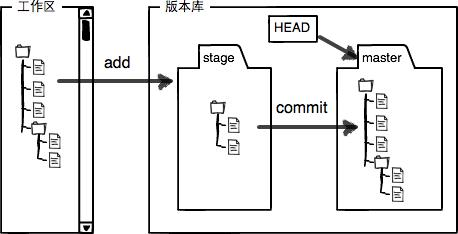
\includepdf{chart/1.pdf}
\newpage
\thispagestyle{empty}
\mbox{}
\newpage
\includepdf[pages={1,2}]{chart/2.pdf} 
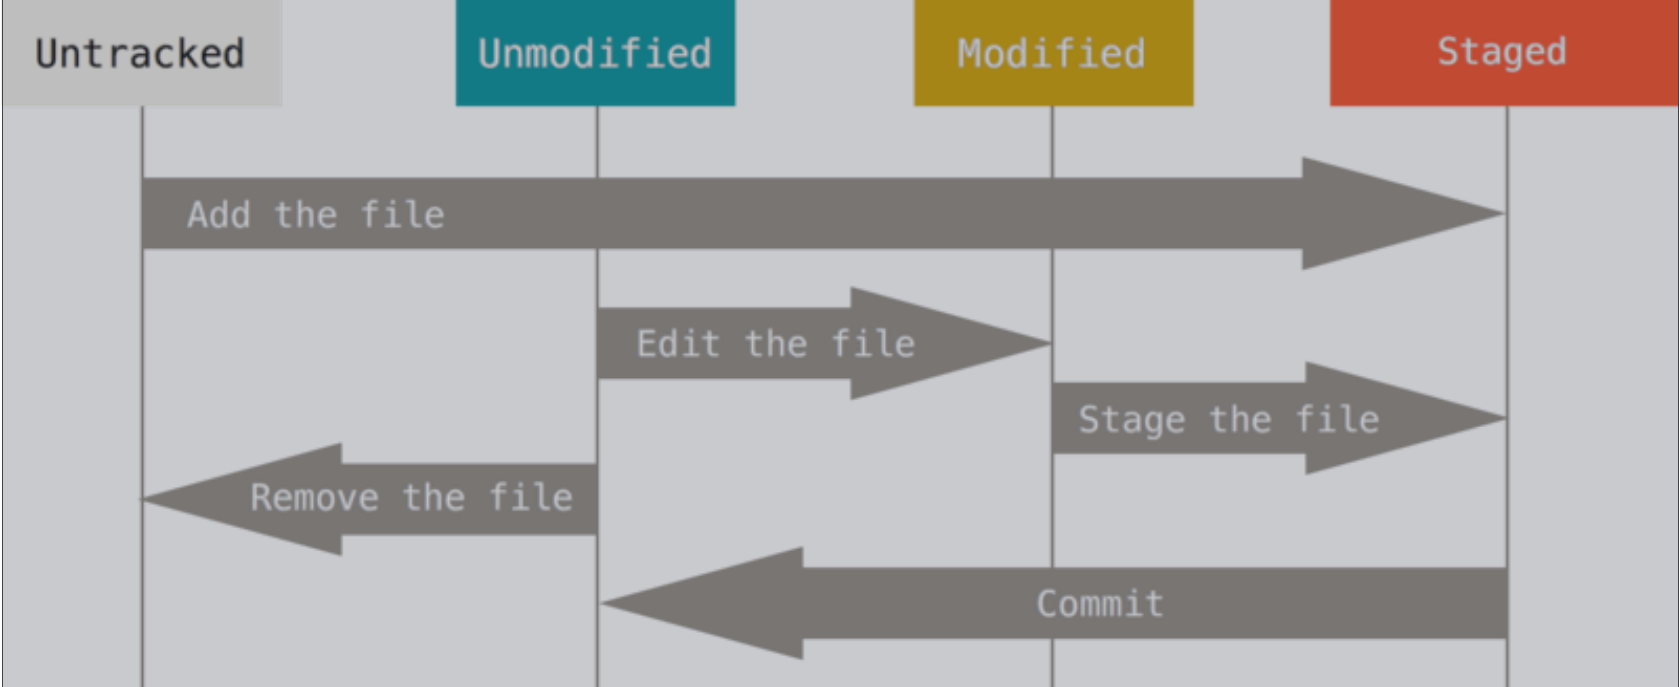
\includepdf{chart/3.pdf} 
\newpage
\mbox{}
\thispagestyle{empty}
\newpage
\includepdf[pages={1,2}]{chart/4.pdf} 
\newpage
\tableofcontents
\thispagestyle{empty}
\newpage
\thispagestyle{empty}
\mbox{}
\newpage

\begin{center}
\sanhao{\textbf{润湿现象的二维数值模拟研究}}
\end{center}

\pagestyle{plain}
\pagenumbering{arabic} %调整页码

\noindent \xiaosihao{\textbf{摘要:}}
\wuhao{固体表面的润湿现象是一种常见自然现象,它在人类生产生活中有着非常广泛的应用,因此
    研究 其内机理有着重要的应用价值。 本文着重用数值模拟的方法研究液滴接触固体
    表面时, 其形状的变化规律。本文假设液滴的形状具有旋转对称性,从而把问题转化
    为液滴中心横截面边界形状的变化问题。进一步基于 Yong 能量泛函, 把横截面边界
    离散为多边形,导出了离散的 Yong 能量泛函, 并结合序列二次规划算法
    Sequential quadratic programming(SQP) 来求解离散能量泛函模型的极小值,从而
    得到模型稳定状态时的能量值及其边界形状。最后通过大量数值实验, 验证了离散模
    型及优化算法的正确性和有效性。}
    
\noindent \xiaosihao{\textbf{关键词:}}
\wuhao{润湿现象; 非线性优化算法; 数值模拟}


\newpage
\begin{center}
\sanhao{\textbf{Two dimensional numerical simulation of wetting phenomenon}}
\end{center}

\noindent \xiaosihao{\textbf{Abstract:}}
\wuhao{The wetting phenomenon of solid surfaces is a common natural phenomenon. It has
a very wide range of applications in human production and life. Therefore, studying 
its internal mechanism has important application value. This paper focuses on 
the method of numerical simulation to study the shape change of droplets when 
they touch the solid surface. This paper assumes that the shape of the droplet 
has rotational symmetry, thus transforming the problem into a change in the shape 
of the boundary shape of the droplet's central cross-section. Further based on 
the Yong energy functional, the cross-sectional boundaries are discretized into 
polygons, the discrete Yong energy functional is derived, and combined with the 
sequential quadratic programming algorithm (SQP) to solve the minimum value of 
the discrete energy functional model, thus The energy value and its boundary 
shape at the steady state of the model are obtained. Finally, through a large 
number of numerical experiments, the correctness and effectiveness of the 
discrete model and optimization algorithm are verified.}

\noindent \xiaosihao{\textbf{Key words:}}
\wuhao{Wetting phenomenon; Nonlinear optimization algorithm; Numerical simulation}



\newpage

\section{第一章 绪论}
\subsection{简介}
润湿现象是一种自然界中常见的现象,指的是固体与液体两个表面相接触时,液体会顺着固
体表面延展开的现象。它的存在影响着人类生产生活的方方面面,如化工(油墨, 杀虫剂等);
汽车制造 (轮胎附着力加强防止在结冰地面打滑等); 土壤学 (液体渗透到多孔岩石中等);
化妆品 (面霜, 睫毛膏, 身体乳等) ,更多应用见 \cite{meng} 有更多的描述。

润湿现象的理论研究最早始于英国科学家 Thomas Yong(1773-1829),他在文章
\cite{young} 中提出的 Yong 方程, 奠定了整个润湿现象研究的理论基础,但当时关注的
人并不是很多。随着科学的不断进步,越来越多人开始关注这个现象,并且对表面张力做了
一定的研究。关于润湿现象有两个经典的模型构建,分别是 Wenzel 模型 \cite{wenzel} 和
Cassie-Baxter 模型 \cite{cassie}。中国对于润湿现象的研究到20世纪才有,
Li\cite{li} 对润湿现象的发展进行了总结,Qin\cite{qin} 构建了润湿现象的表面能量平衡方
程。但是以上的工作大部分是对润湿现象模型的建立,缺乏对模型优化的讨论。

液滴滴落在一个均匀平滑的固体表面上时,会出现两种现象。一种是液滴完全覆盖在固
体表面上,例如将水滴在纸面。另一种则是本篇文章讨论的情况,液滴与固体表面
仍会形成一定的角度并留在固体表面上,例如雨后荷叶上的液滴

\begin{figure}[H]
	\centering
	
\includegraphics[width=0.3\linewidth]{figure/lotus.jpg}
	\caption{雨后荷叶上的液滴}
	\label{fig:7}
\end{figure}

\noindent 其中在气、液、固三个表面所形成的交点处作气-液界面的切线,其与固体表
面的夹角我们称之为接触角,通常用$\theta$表示。

\begin{figure}[H]
	\centering
	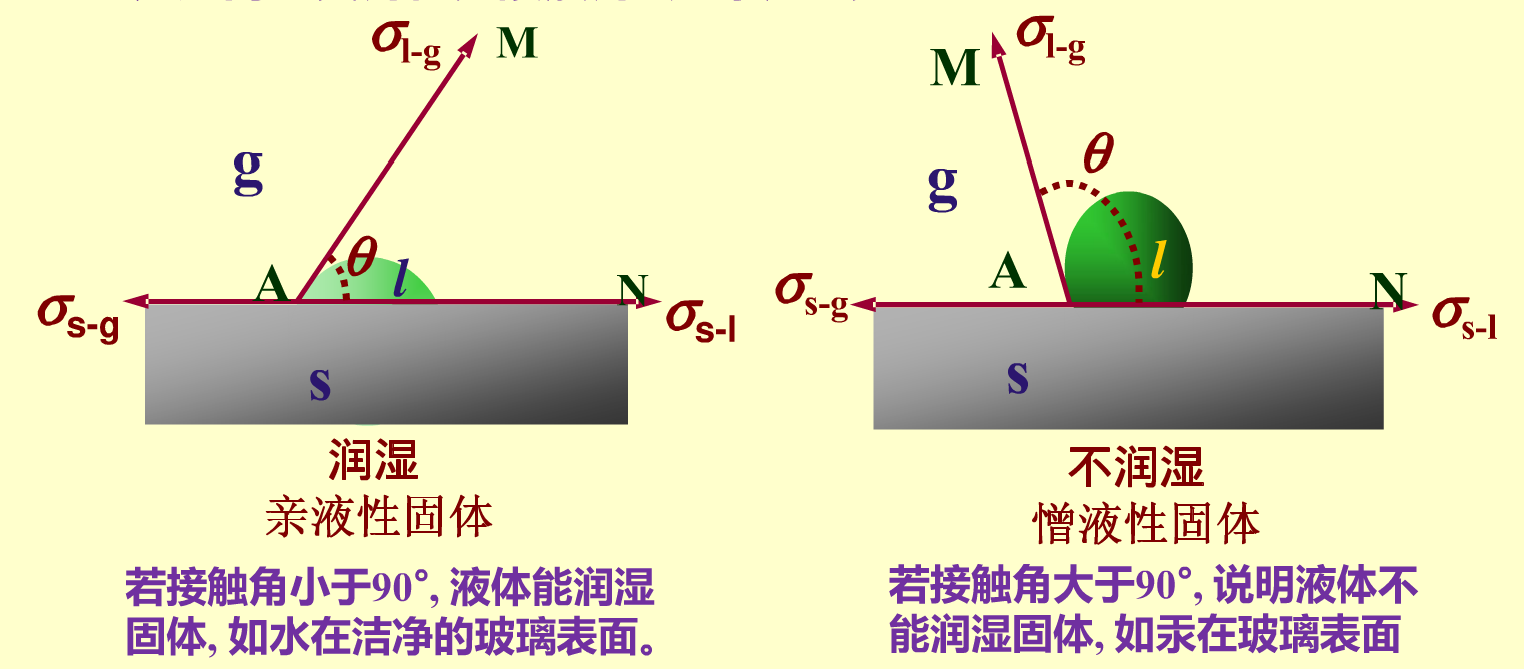
\includegraphics[width=0.5\linewidth]{figure/contact-angel.png}
	\caption{接触角}
	\label{fig:8}
\end{figure}

接触角大小可以很好的的反应出液体对固体的润湿性能,接触角越大则润湿性能越不好,
接触角越小润湿性能越好。通常当 $\theta > 90^{\circ}$ 称为不润湿, $\theta < 90^{\circ}$
称为润湿。

表面自由能是物体表面分子间作用力的体现,与固体表面的润湿性能密切相关。这也是润
湿现象发生的原因,为改变物体表面的润湿性能,使其更好的满足我们的需求,更有效的
应用于各行各业, 润湿现象已经是一个多学科交叉的热点问题.本
文将通过数值实验对润湿现象进行模拟,以此来更好的了解润湿现象。

\subsection{预备知识}

\subsubsection{Newton法解方程组}
由 Taylor 展开可将方程组 $\bfF(\bfx)=0$ ,变成
\begin{equation*}
\bfF(\bfx) \approx \bfF\left(\bfx^{k}\right)+
\bfF'\left(\bfx^{k}\right)\left(\bfx-\bfx^{k}\right)=0,
\end{equation*}
当$\bfF'\left(\bfx^{k}\right)$非奇异时,令$\bfx = \bfx^{k+1}$,得
\begin{equation*}
\bfx^{k+1}=\bfx^{k}-\bfF^{\prime}\left(\bfx^{k}\right)^{-1} \bfF\left(\bfx^{k}\right)(k=0,1, \cdots),
\end{equation*}
这就是牛顿法,其中
\begin{equation*}
\bfF^{\prime}\left(\bfx^{k}\right)=\left(\begin{array}{cccc}
\frac{\partial f_{1}\left(\bfx^{k}\right)}{\partial x_{1}} &
\frac{\partial f_{1}\left(\bfx^{k}\right)}{\partial x_{2}} &
\cdots & \frac{\partial f_{1}\left(\bfx^{k}\right)}{\partial x_{n}} \\
\frac{\partial f_{2}\left(\bfx^{k}\right)}{\partial x_{1}} &
\frac{\partial f_{2}\left(\bfx^{k}\right)}{\partial x_{2}} &
\cdots & \frac{\partial f_{2}\left(\bfx^{k}\right)}{\partial x_{n}} \\
\cdots & \cdots & \cdots & \cdots \\
\frac{\partial f_{n}\left(\bfx^{k}\right)}{\partial x_{1}} &
\frac{\partial f_{n}\left(\bfx^{k}\right)}{\partial x_{2}} &
\cdots & \left.\frac{\partial f_{n}\left(\bfx^{k}\right)}{\partial x_{n}}\right)
\end{array}\right),
\end{equation*}
是$F$在$\bfx^k$处的雅克比矩阵,$x_i$是$\bfx^k$的第i个分量。

牛顿法的步骤为先给初始点$\bfx^0$,计算$\bfF(\bfx^k)$
和$\bfF^{\prime}\left(\bfx^{k}\right)$,然后解方程组
\begin{equation*}
\bfF^{\prime}\left(\bfx^{k}\right) \Delta \bfx^{k}=-\bfF\left(\bfx^{k}\right),
\end{equation*}
此方程组称为牛顿方程,求得解$\Delta \bfx^{k}$,于是由
\begin{equation*}
\bfx^{k+1}=\bfx^{k}+\Delta \bfx^{k},
\end{equation*}
依次求出$\bfx^1,\bfx^2,\ldots$。

\subsubsection{Kuhn-Tucker(KT)条件}
KT条件是非线性规划领域中最重要的理论成果\cite{yun},是某点为最优点的必要条件,
一般来说它并不是充分条件,但是对于凸优化来说,它即是最优点的必要条件,同时也是充分条件。

对于非线性规划问题
\begin{align}\label{nl}
\begin{array}{rlrl}
\min & f(\mathbf{X}) & & \\
& h_{i}(\mathbf{X})=0, & & i=0,1, \cdots, m_e \\
& g_{j}(\mathbf{X}) \geqslant 0, & & j=m_{e+1},m_{e+2}, \cdots, m
\end{array},
\end{align}
\noindent 其KT条件如下:

设$\bfX^*$为非线性规划式$\ref{nl}$的极小点,而且$\bfX^*$点的所起作用约束的梯度
$\nabla h_{i}\left(\mathbf{X}^{*}\right)(i=1,2, \cdots, m)$
和$\nabla g_{j}\left(\bfX^{*}\right)(j \in J)$线性无关($J$为起作用约
束下标的集合),则存在向量

$$\boldsymbol{\lambda}^{*}=\left(\lambda_{0}^{*}, \lambda_{1}^{*}, \cdots, \lambda_{m}^{*}\right)^{\mathrm{T}},$$

\noindent 使下述条件成立

\begin{align*}
&\nabla f\left(\boldsymbol{x}^{*}\right)-\sum_{i=0}^{m_e} \lambda_{i}^{*} \nabla h_{i}\left(\boldsymbol{x}^{*}\right)-
\sum_{j=m_{e+1}}^{m} \lambda_{j}^{*} \nabla g_{j}\left(\boldsymbol{x}^{*}\right)=0 \\
&\lambda_{j}^{*} g_{j}\left(\boldsymbol{X}^{*}\right)=0, \quad j=m_{e+1},m_{e+2}, \cdots, m \\
&\lambda_{j}^{*} \geqslant 0, \quad \quad j = m_{e+1},m_{e+2}, \cdots, m\\
& g_{j}(\mathbf{X}) \geqslant 0,  j=m_{e+1},m_{e+2}, \cdots, m\\
& h_{i}(\mathbf{X})=0,  i=0,1, \cdots, m_e ,
\end{align*}

\noindent 满足上述条件的点称为K-T点

\subsubsection{拟牛顿算法的Hessain矩阵更新}
在高数中,学过泰勒公式,如下
  \begin{equation*}
  f(x)=\frac{f\left(x_{0}\right)}{0 !}+\frac{f^{\prime}\left(x_{0}\right)}{1 !}\left(x-x_{0}\right)+
  \frac{f^{\prime \prime}\left(x_{0}\right)}{2 !}\left(x-x_{0}\right)^{2}+\ldots+
  \frac{f^{(n)}\left(x_{0}\right)}{n !}\left(x-x_{0}\right)^{n}+R_{n}(x),
  \end{equation*}
对于拟牛顿法来说,构造二次模型。如下

\begin{equation*}
f(\bfX)=f(\bfX_{i+1})+(\bfX-\bfX_{i+1})^{T} \nabla
f(\bfX_{i+1})+\frac{1}{2}(\bfX-\bfX_{i+1})^{T} \bfH(\bfX-\bfX_{i+1})+o(\bfX-\bfX_{i+1}),
\end{equation*}
忽略高阶无穷小部分,进行求导得到

\begin{equation*}
\nabla f(\bfX) \approx \nabla f(\bfX_{i+1})+\bfH(\bfX-\bfX_{i+1}),
\end{equation*}
令$\bfX = \bfX_i$,那么得到

\begin{equation*}
\bfH^{-1}[\nabla f(\bfX_{i+1})-\nabla f(\bfX_{i})] \approx \bfX_{i+1}-\bfX_{i},
\end{equation*}
我们用$\bfB_i$序列对 Hessian 矩阵的逆矩阵进行逼近

\begin{equation*}
\bfB_{i+1}[\nabla f(\bfX_{i+1})-\nabla f(\bfX_{i})] \approx \bfX_{i+1}-\bfX_{i},
\end{equation*}
这个方程就是拟牛顿方程。所以最关键的问题是如何得到每一步的$\bfB_{i+1}$。

假设有如下迭代

\begin{align*}
&\bfB_{i+1}=\bfB_{i}+\bfE_{i}\\
&\bfE_{i}=m \bfV \bfV^{T}+n \bfW \bfW^{T},
\end{align*}
其中$m$和$n$均为实数,$\bfV,\bfW$均为$\bfN$维向量,带入上述拟牛顿方程,有如下推导

\begin{align*}
\bfB_{i+1}\left[\nabla \bff\left(\bfX_{i+1}\right)-\nabla \bff\left(\bfX_{i}\right)\right] 
&=\left(\bfB_{i}+\bfE_{i}\right)\left[\nabla \bff\left(\bfX_{i+1}\right)-\nabla \bff\left(\bfX_{i}\right)\right] \\
&=\left(\bfB_{i}+m \bfV \bfV^{T}+n \bfW \bfW^{T}\right)\left[\nabla \bff\left(\bfX_{i+1}\right)-\nabla \bff\left(\bfX_{i}\right)\right] \\
&=\bfX_{i+1}-\bfX_{i},
\end{align*}
进一步有

\begin{equation*}
\bfB_{i}\left[\nabla \bff\left(\bfX_{i+1}\right)-\nabla \bff\left(\bfX_{i}\right)\right]+
m \bfV \bfV^{T}\left[\nabla \bff\left(\bfX_{i+1}\right)-\nabla \bff\left(\bfX_{i}\right)\right]+
n \bfW \bfW^{T}\left[\nabla \bff\left(\bfX_{i+1}\right)-\nabla \bff\left(\bfX_{i}\right)\right]=\bfX_{i+1}-\bfX_{i},
\end{equation*}
接下来,我们重新记一下符号,设

\begin{equation*}
\begin{array}{l}
\bft_{i}=\nabla \bff\left(\bfX_{i+1}\right)-\nabla \bff\left(\bfX_{i}\right) \\
\bfs_{i}=\bfX_{i+1}-\bfX_{i}
\end{array},
\end{equation*}
那么得到

\begin{equation*}
\bfB_{i} \bft_{i}+\bfm \bfV \bfV^{T} \bft_{i}+n \bfW \bfW^{T} \bft_{i}=
\bfB_{i} \bft_{i}+\bfV\left(\bfm \bfV^{T} \bft_{i}\right)+\bfW\left(n \bfW^{T} \bft_{i}\right)=\bfs_{i},
\end{equation*}

现在只要我们求出$m,n,\bfV,\bfW$,那么问题也就解决了。那么为了更容易看出结论,继续作如下变换

\begin{equation*}
\bfV\left(m \bfV^{T} \bft_{i}\right)+\bfW\left(n \bfW^{T} \bft_{i}\right)=\bfs_{i}-\bfB_{i} \bft_{i},
\end{equation*}
那么只需要如下几个条件成立就可以了

\begin{align*}
&\bfV=\bfs_{i}\\
&m \bfV^{T} \bft_{i}=1\\
&\bfW =\bfB_i \bft_i\\
&n \bfW^{T} \bft_{i}=-1,
\end{align*}
带入原式最终得到

\begin{align*}
\bfB_{i+1} &= \bfB_i+\frac{\bfs_i \bfs_{i}^{T}}{\bfs_i^{T} \bft_i}-
\frac{\bfB_i \bft_i(\bfB_i \bft_i)^T}{(\bfB_i \bft_i)^T \bft_i} \\
&=\bfB_i+\frac{\bfs_i \bfs_{i}^{T}}{\bfs_i^{T} \bft_i}-
\frac{\bfB_i \bft_i \bft_i^T \bfB_i}{(\bfB_i \bft_i)^T \bft_i},
\end{align*}

\subsubsection{弧长与面积}
设平面曲线的参数方程为
\begin{align}\label{cure}
\left\{\begin{array}{ll}
x=x(t) & t \in\left[T_{1}, T_{2}\right] \\
y=y(t) & t \in\left[T_{1}, T_{2}\right]
\end{array}\right.
\end{align}
若参数方程$\ref{cure}$的$x'(t)$,$y'(t)$在$[T_{1}, T_{2}]$上连续,
且$\left[x^{\prime}(t)\right]^{2}+\left[y^{\prime}(t)\right]^{2} \neq 0$,
则他所确定的曲线称为光滑曲线,其弧长\cite{chen}为
\begin{equation*}
l=\int_{T_{1}}^{T_{2}} \sqrt{\left[x^{\prime}(t)\right]^{2}+\left[y^{\prime}(t)\right]^{2}} d t,
\end{equation*}
\noindent 面积为
\begin{align*}
S &=\int_{a}^{b} f(x) d x \\
 &=\int_{T_{1}}^{T_{2}}\left|y(t) x^{\prime}(t)\right| d t.
\end{align*}

\subsection{本文的主要工作和后续安排}
本文主要是建立和优化二维液滴润湿现象模型,安排如下:

第一章主要介绍润湿现象的物理意义、研究背景和发展现状,简要介绍后续会用到的一些
基本知识。

第二章研究表面张力,液滴样貌和接触角来确定表面自由能和约束条件,建立数学模型,并进行离散化。

第三章建立非线性约束化理论,首先将整个算法进行整体的描述,具体分为三个部分:搜寻方向、步长、以及Hessean矩阵的更新。整体描述后我们再进行具体的推导和分析。

第四章进行数值模拟,控制不同的单一变量,来分析模型和优化算法的正确性。


\newpage

\section{第二章 液滴模型建立}
\subsection{数学理论推导}
研究不同表面张力,液滴形状及接触角来确定总表面自由能和约束条件。对液滴在固体界面平衡状态做受力分析
\begin{figure}[H]
	\centering
	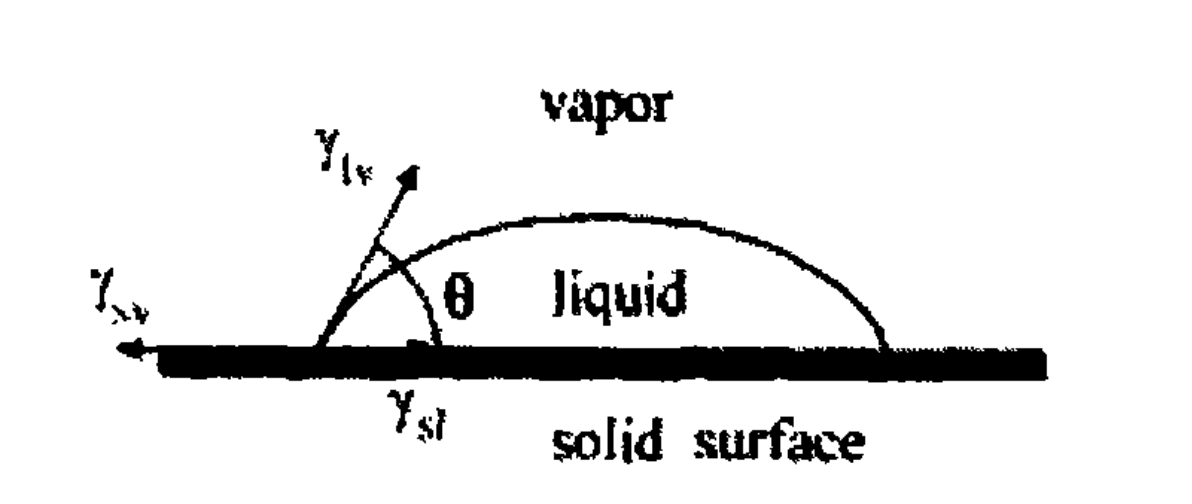
\includegraphics[width=0.5\linewidth]{figure/force.png}
	\label{fig:1}
\end{figure}
\noindent 其中$\gamma_{LV},\gamma_{SL},\gamma_{SV}$分别表示液-气,固-液,固-气表面的张力,
$\theta$则表示接触角。由于液滴保持平衡状态,所以液-气表面张力在固液交界面的分力,
和固-液,固-气表面的张力三个力的和必须为零,便得到

\begin{equation}\label{yong}
\gamma_{L V} \cos \theta=\gamma_{S V}-\gamma_{S L},
\end{equation}

\noindent $\ref{yong}$便为著名的Yong方程\cite{young}。

由于表面自由能等于张力乘以面积\cite{qin},因此系统总能量如下

\begin{equation*}
\varepsilon=\int_{\Sigma_{SL}} (\gamma_{SL}-\gamma_{SV}) d S+\int_{\Sigma_{LV}} \gamma_{LV} d S,
\end{equation*}

\noindent 其中$\varepsilon$为自由能,$\Sigma_{SL},\Sigma_{LV}$分别为固-液,液-气交界面。

由于模型简化为二维情况,因此公式变为

\begin{equation*}
\varepsilon=\gamma_{SL}A_{LV}+(\gamma_{SL}-\gamma_{SV})A_{SL},
\end{equation*}

\noindent 其中$A_{LV},A_{SL}$分别为固-液,液-气交界处长度。

将Yong方程带入到上述公式中,便得到

\begin{equation*}
\frac{\varepsilon}{\gamma_{LV}}=A_{LV}-\cos \theta A_{SL},
\end{equation*}

\noindent 令$\frac{\varepsilon}{\gamma_{LV}} = F$为我们寻找的极小函数。

由于液滴体积不会发生改变,因此带有约束条件

\begin{equation*}
\oint dv = v_0,
\end{equation*}

\noindent 其中$v_0$为初始液滴体积。

最终建立液滴模型问题

\begin{equation*}
\min  F = A_{LV}-\cos \theta A_{SL} ,\\
\end{equation*}
使得
\begin{equation*}
\oint dv = v_0,
\end{equation*}



\subsection{模型离散}
给定在[0,T]上的N+1个起始点$(x_{0},y_{0}),(x_{1},y_{1}),\cdots,(x_{N},y_{N})$用
来描述液滴初试的样貌,每一段参数曲线可表示为$p_{i}(t)=(X_{i}(t),Y_{i}(t))$
\begin{equation*}
X_{i}(t)=(1-t)x_{i}+tx_{i+1}, t \in [0,1],i=0,1,\dots,N.
\end{equation*}

\begin{equation*}
Y_{i}(t)=(1-t)y_{i}+ty_{i+1}, t \in [0,1],i=0,1,\dots,N.
\end{equation*}

\noindent $ A_{SL},A_{LV}$可以表示为
\begin{equation*}
A_{SL}=\sum_{i=0}^{N-1}\int_{0}^{1}(x_{i+1}-x_{i})dt=x_{N}-x_{0}.
\end{equation*}

\begin{equation*}
A_{LV}=\sum_{i=0}^{N-1}\int_{0}^{1}\sqrt{(y_{i+1}-y_{i} )^2+(x_{i+1}-x_{i})^2}dt=
\sum_{i=0}^{N-1}\sqrt{(y_{i+1}-y_{i} )^2+(x_{i+1}-x_{i})^2}.
\end{equation*}

\noindent 因此极小能量函数可以表示为
\begin{align*}
F &= A_{LV}-\cos\theta A_{SL} \\
  &=\sum_{i=0}^{N-1}\sqrt{(y_{i+1}-y_{i} )^2+(x_{i+1}-x_{i})^2} - \cos \theta (x_{N}-x_{0}),
\end{align*}

接下来求其梯度值

\begin{align*}
\frac{\partial F}{\partial x_i} = \left\{\begin{array}{ll}
\frac{x_{i}-x_{i+1}}{h_{i}} - \frac{x_{i-1}-x_{i}}{h_{i-1}} & i=1,2,\ldots,N-1 \\
\frac{x_0-x_1}{h_0} + \cos\theta & i=0 \\
\frac{x_N-x_{N-1}}{h_{N-1}} - \cos\theta & i=N
\end{array}\right.
\end{align*}

\begin{align*}
\frac{\partial F}{\partial y_i} = \left\{\begin{array}{ll}
\frac{y_{i}-y_{i+1}}{h_{i}} - \frac{y_{i-1}-y_{i}}{h_{i-1}} & i=1,2,\ldots,N-1 \\
\frac{y_0-y_1}{h_0} & i=0 \\
\frac{y_N-y_{N-1}}{h_{N-1}} & i=N
\end{array}\right.
\end{align*}

约束面积S为:
\begin{equation*}
S=\sum_{i=0}^{N-1}\dfrac{(x_{i+1}-x_{i})(y_{i+1}+y_{i})}{2}=S_{0},
\end{equation*}

边界条件为:
\begin{equation*}
y_{0}=0,y_{N}=0.
\end{equation*}

实现的代码详见附录。

\newpage
\mbox{}
\newpage

\section{第三章 非线性约束优化理论}
接下来我们介绍本次模型优化所使用的算法SQP\cite{kraft}。该算法主要是来解决非线性
约束的最小值问题.主要思想为:在求解约束优化问题时,在每一初始迭代点构造一个二
次规划子问题,将该子问题的解作为迭代搜索的方向,并选取相应的效益函数确定迭代搜
索的步长; 通过求解上述子问题修正迭代点,直到二次规划的结果逼近原非线性规划问题的最优解。

\subsection{问题模型}
\begin{equation}\label{iq}
\min _{x \in R^{n}} f(\bfx)
\end{equation}
使得
\begin{equation*}
\begin{array}{c}
g_{j}(\bfx)=0, \quad j=0, \ldots, m_{e} \\
g_{j}(\bfx) \geq 0, \quad j=m_{e}+1, \ldots, m \\
\quad \bfx_{l} \leq \bfx \leq \bfx_{h}
\end{array}
\end{equation*}
其中$f: R^{n} \rightarrow R$为目标函数,$ g_j(\bfx):R^{n} \rightarrow R$为约束条
件,都假设为连续可微.

\subsection{算法结构}
主要过程为,给定一个初始解$\bfx^0$

\begin{itemize}
\item 确定搜索方向$\bfd^k$,也就是依照某种规则,构造目标函数f在$\bfx^k$处的下降方向
\item 确定搜索步长$\alpha^k$,使目标函数值有某种意义上的下降
\item 令
\begin{equation}\label{step}
\bfx^{k+1}:=\bfx^k+\alpha^k \bfd^k,
\end{equation}
若$\bfx^{k+1}$满足终止性条件,则停止迭代,得到近似最优解$\bfx^{k+1}$;否则重复以上步骤
\end{itemize}

\subsubsection{搜寻方向}
搜寻方向是通过一个二次规划子问题来决定,其由该问题的lagrange函数的二次逼近

\begin{equation}\label{lf}
L(\bfx, {\boldsymbol \lambda})=f(\bfx)-\sum_{j=0}^{m} \lambda_{j} g_{j}(\bfx)=
f(\bfx) - {\boldsymbol \lambda}^T \bfg(\bfx),
\end{equation}

\noindent 和约束条件的线性逼近来决定

该二次规划的标准形式可以写为

\begin{equation}\label{qp}
\min _{d \in R^{n}} \frac{1}{2} \bfd^{T} \bfB^{k} \bfd+\nabla {\boldsymbol f\left(\bfx^{k}\right)} \bfd
\end{equation}

\noindent 使得

\begin{equation*}
\nabla \bfg_{j}\left(\bfx^{k}\right) \bfd+g_{j}\left(\bfx^{k}\right)=0, \quad j=0, \ldots, m_{c}
\end{equation*}

\begin{equation*}
\nabla \bfg_{j}\left(\bfx^{k}\right) \bfd+g_{j}\left(\bfx^{k}\right) \geq 0, \quad j=m_{e}+1, \ldots, m.
\end{equation*}

其中${\boldsymbol \lambda}=(\lambda_0,\lambda1,\ldots,\lambda_m)^T$,$\bfg(\bfx)=
(g_0(\bfx),g_1(\bfx),\ldots,g_m(\bfx))^T$,$\bfB:=\nabla_{x x}^{2} L(\bfx, {\boldsymbol \lambda})$
即为拉格朗日函数$\ref{lf}$的 Hessian 阵,注意这里的$\nabla \bfg_{j}(\bfx),\nabla f(\bfx)$都为行向量。

上述搜寻方向的选择最早由Wilson\cite{wilson}在1963年推导出来。
\subsubsection{步长}
我们通过外点罚函数法来确定步长,外点罚函数法的基本思想是构造辅助函数
\begin{equation*}
F_{\varrho}: R^{n} \rightarrow R \quad(\mu>0),
\end{equation*}
函数$F_{\varrho}$在可行域D的内部取值与原问题$\ref{iq}$的目标函数$f$一样,而在可
行域外部取值远远大于目标函数$f$.

换言之,对可行域外部的点的目标函数值加以惩罚,使得无约束问题$\min F_{\varrho}(x)$的
解是约束问题$\ref{iq}$的近似解,且当惩罚因子足够大的时候,问题$\min F_{\varrho}(x)$的
解$\bfx(\varrho)$趋于约束问题$\ref{iq}$的解。

对于$\ref{iq}$我们可以定义辅助函数
\begin{equation*}
F(\bfx, \varrho)=f(\bfx)+\varrho P(\bfx),
\end{equation*}
其中$P(x)$具有如下形式

\begin{equation*}
P(\bfx)=\sum_{i=1}^{m} \phi\left(g_{i}(\bfx)\right)+\sum_{j=1}^{l} \psi\left(h_{j}(\bfx)\right),
\end{equation*}
连续函数$\phi$和$\psi$满足

\begin{equation*}
\phi(y)\left\{\begin{array}{l}
=0, y \geq 0 \\
>0, y<0
\end{array}, \quad \psi(y)\left\{\begin{array}{l}
=0, y=0 \\
>0, y \neq 0
\end{array}\right.\right.
\end{equation*}
因此我们定义如下惩罚函数,参数的选择由Powell\cite{powell}得出,

\begin{equation*}
\phi(\bfx ; \varrho):=f(\bfx)+\sum_{j=0}^{m_{e}+1} \varrho_{j}\left|g_{j}(\bfx)\right|+
\sum_{j=m_{e}+1}^{m} \varrho_{j}\left|g_{j}(\bfx)\right|_{-},
\end{equation*}
其中$\left|g_{j}(\bfx)\right|_{-}:=\left|\min (0, g_{j}(\bfx)) \right|$,$e_j$为惩罚参数

优化函数为$\varphi : R^1 \rightarrow R^1$
\begin{equation*}
\varphi(\alpha):=\phi\left(\bfx^{k}+\alpha \bfd^{k}\right),
\end{equation*}
$e_j$惩罚参数的更新根据下面的式子

\begin{equation}\label{1}
\varrho_{j}:=\max \left(\frac{1}{2}\left(e_{j}^{-}+\left|\lambda_{j}\right|\right),
\left|\lambda_{j}\right|\right), \quad j=0, \ldots, m.
\end{equation}

其中$\lambda_{j}$表示在二次规划中第j个约束条件的lagrange乘子,$e_{j}^{-}$是上一次迭代的第j个惩罚参数,开始时$e^0_j=0$


\subsubsection{B矩阵的更新}
这里我们用BFGS来更新我们的矩阵$\bfB$,为了保证正定性我们加入参量$\theta$,参量的
选择由Powell\cite{powell}得出,
\begin{equation*}
\bfB^{k+1}:=\bfB^{k}+\frac{\bfq^{k}\left(\bfq^{k}\right)^{T}}{\left(\bfq^{k}\right)^{T} \bfs^{k}}-
\frac{\bfB^{k} \bfs^{k}\left(\bfs^{k}\right)^{T} \bfB^{k}}{\left(\bfs^{k}\right)^{T} \bfB^{k} \bfs^{k}},
\end{equation*}
其中

\begin{equation*}
\bfs^{k}:=\bfx^{k+1}-\bfx^{k}=\alpha^{k} \bfd^{k},
\end{equation*}

\begin{equation*}
\bfq^{k}:=\theta^{k} {\boldsymbol \eta}^{k}+\left(1-\theta^{k}\right) \bfB^{k} \bfs^{k},
\end{equation*}
这里的$\eta^{k}$为前后两次迭代lagrange函数梯度的差值

\begin{equation*}
{\boldsymbol \eta}^{k}:=\nabla_{x} \bfl\left(\bfx^{k+1}, {\boldsymbol\lambda}^{k}\right)-
\nabla_{x} \bfl\left(\bfx^{k}, {\boldsymbol\lambda}^{k}\right),
\end{equation*}

\begin{equation*}
\theta^{k}:=\left\{\begin{array}{ll}
1, & \text { if }\left(\bfs^{k}\right)^{T} {\boldsymbol \eta}^{k} \geq 
0.2\left(\bfs^{k}\right)^{T} \bfB^{k} \bfs^{k} \\
\frac{0.8\left(\bfs^{k}\right)^{T} \bfB^{k}\bfs^{k}}{\left(\bfx^{k}\right)^{T} \bfB^{k}\bfx^{k}-
\left(\bfx^{k}\right)^{T} {\boldsymbol \eta}^{k}}, & \text { otherwise }
\end{array}\right.
\end{equation*}

\subsection{算法推导}
首先原问题为

\begin{equation*}
\min _{x \in R^{n}} f(\bfx)
\end{equation*}
使得
\begin{equation*}
\begin{array}{c}
g_{j}(\bfx)=0, \quad j=0, \ldots, m_{e} \\
g_{j}(\bfx) \geq 0, \quad j=m_{e+1}, \ldots, m .
\end{array}
\end{equation*}
建立其Lagrange函数

\begin{equation}\label{la}
L(\bfx, \boldsymbol{ \lambda})=f(\bfx)-\sum_{i=0}^{m} \lambda_{i}  g_{i}(\bfx)
=f(\bfx)-\boldsymbol{\lambda}^T  \bfg(\bfx),
\end{equation}
其中$\boldsymbol{\lambda} = (\lambda_0,\lambda_1,\ldots,\lambda_{m})^T$
为lagrange乘子向量.$\bfg(\bfx) = (g_0(\bfx),g_1(\bfx),\ldots,g_{m}(\bfx))^T$
约束函数$\bfg(\bfx)$的Jacobi矩阵记为
\begin{equation*}
\bfA^T(\bfx)=\nabla \bfg(\bfx)=\left(\begin{array}{c}
\nabla \bfg_{0}(\bfx) \\
\vdots \\
\nabla \bfg_{m}(\bfx).
\end{array}\right)
\end{equation*}
其中$\nabla \bfg_{i}(\bfx)$和$\nabla \bff(\bfx)$都为行向量,
由k-t条件可知道,对$\ref{la}$求导都应为0,可得下列方程组

\begin{equation}\label{grad}
\nabla L(\bfx, \boldsymbol{ \lambda})=\left[\begin{array}{l}
\nabla_{x} L(\bfx, \boldsymbol{ \lambda})) \\
\nabla_{\lambda} L(\bfx, \boldsymbol{ \lambda})
\end{array}\right]=\left[\begin{array}{l}
\nabla f(\bfx)^T-\mathrm{A}(\bfx)\boldsymbol{\lambda} \\
\bfg(\bfx)
\end{array}\right]= \emph{0}.
\end{equation}
且$\lambda_i \geq 0,i \in \{m_{e+1},\ldots,m\}$

现在用newton法解$n+m+1$维的方程组$\ref{grad}$

\begin{equation}\label{new1}
J\left(\bfx^{k}, \boldsymbol{\lambda}^{k}\right)\left(\begin{array}{c}
\Delta \bfx \\
\Delta  \boldsymbol{ \lambda}
\end{array}\right)=-\nabla L(\bfx^k, \boldsymbol{ \lambda}^k),
\end{equation}

\begin{equation}\label{new2}
\left(\begin{array}{c}
\bfx^{k+1} \\
\boldsymbol{ \lambda}^{k+1}
\end{array}\right):=\left(\begin{array}{c}
\bfx^{k} \\
\boldsymbol{ \lambda}^{k}
\end{array}\right)+\left(\begin{array}{c}
\Delta \bfx \\
\Delta \boldsymbol{ \lambda}
\end{array}\right).
\end{equation}
其中$\bfJ\left(\bfx^{k}, \boldsymbol{\lambda}^{k}\right)$为
$\nabla L(\bfx^k, \boldsymbol{ \lambda}^k)$的jacobi矩阵

\begin{equation*}
\bfJ\left(\bfx^{k}, \boldsymbol{\lambda}^{k}\right)=\left(\begin{array}{cc}
\bfB\left(\bfx^{k}, \boldsymbol{ \lambda}\right) & -\bfA\left(\bfx^{k}\right) \\
\bfA\left(\bfx^{k}\right)^{T} & 0
\end{array}\right).
\end{equation*}

\begin{equation*}
\bfB\left(\bfx^{k}, \boldsymbol{\lambda}^{k}\right)=\nabla_{x}^{2} f\left(\bfx^{k}\right)-
\sum_{j=0}^{m} \boldsymbol{\lambda}_{j}^{k} g_{j}\left(\bfx^{k}\right).
\end{equation*}
为Lagrange函数的Hessian矩阵,将$\ref{new1}$和$\ref{new2}$展开写变为

\begin{equation}\label{fin}
\left(\begin{array}{cc}
\bfB\left(\bfx^{k}, \boldsymbol{\lambda}^{k}\right) & -\bfA\left(\bfx^{k}\right) \\
\bfA\left(\bfx^{k}\right)^{T} & 0
\end{array}\right)\left(\begin{array}{c}
\bfd \\
\boldsymbol{\lambda}^{k+1}
\end{array}\right)=\left(\begin{array}{c}
-\nabla \bff\left(\bfx^{k}\right) \\
-\bfg\left(\bfx^{k}\right)
\end{array}\right),
\end{equation}

\begin{equation*}
\bfx^{k+1}:=\bfx^{k}+\bfd,
\end{equation*}

而二次规划问题

\begin{equation}\label{qp}
\min _{d \in R^{n}} \frac{1}{2} \bfd^{T} \bfB^{k} \bfd+\nabla {\boldsymbol f\left(\bfx^{k}\right)} \bfd 
\end{equation}
使得

\begin{align*}
\nabla \bfg_{j}\left(\bfx^{k}\right) \bfd+g_{j}\left(\bfx^{k}\right)&=0, \quad j=0, \ldots, m_{e}  \\
\nabla \bfg_{j}\left(\bfx^{k}\right) \bfd+g_{j}\left(\bfx^{k}\right) &\geq 0, \quad j =m_{e}+1, \ldots, m
\end{align*}
的KT条件与$\ref{fin}$一样,因此两个问题等价,原问题转换文等价的二次规划问题$\ref{qp}$

\subsection{qp问题解决}
二次规划(qp)一般形式为
\begin{equation}\label{qp}
\min \quad f(\bfx)=\frac{1}{2} \bfx^{T} \bfQ \bfx+\bfq^{T} \bfx
\end{equation}
使得
\begin{align*}
\bfa_{i}^{T} \bfx-b_{i} & \geq 0, \quad i \in I=\left\{0,1, \cdots, m_{e}\right\} \\
\bfa_{i}^{T} \bfx-b_{i} &=0, i \in E=\left\{m_{e}+1, m_{e}+2, \cdots, m\right\}
\end{align*}
其中$\bfQ$为对称正定,$\bfa_i,\bfq \in R^n$,$b_i \in R$

设$\bfx^*$是问题$\ref{qp}$的最优解,则KT条件,其等价于存在Lagrange乘子$\boldsymbol{\lambda}^*$满足:

\begin{align}\label{ktcon1}
\begin{split}
&\nabla f\left(\bfx^{*}\right)-\sum_{i \in E \cup I} \lambda_{i}^{*} a_{i}=0,\\
&\bfa_{i}^{T} \bfx^{*}-b_{i}=0, \quad i \in E,\\
&\bfa_{i}^{T} \bfx^{*}-b_{i} \geq 0, \quad \lambda_{i}^{*} \geq 0,\\
&\lambda_{i}^{*}\left(\bfa_{i}^{T} \bfx^{*}-b_{i}\right)=0, i \in I,
\end{split}
\end{align}
记

\begin{equation*}
A_{I}=\left(
\begin{array}{c}
a_{1}^{T} \\
a_{2}^{T} \\
\vdots \\
a_{m_e}^{T}
\end{array}\right),
A_{E}=\left(
\begin{array}{c}
a_{m_{e}+1}^{T} \\
a_{m_{e}+2}^{T} \\
\vdots \\
a_{m}^{T}
\end{array}\right),
b_{I}=\left(
\begin{array}{c}
b_{1} \\
b_{2} \\
\vdots \\
b_{m_e}
\end{array}\right),
b_{E}=\left(
\begin{array}{c}
b_{m_{e}+1} \\
b_{m_{e}+2} \\
\vdots \\
b_{m}
\end{array}\right),
A=\left(
\begin{array}{c}
A_{I} \\
A_{E} \\
\end{array}\right).
\end{equation*}
则$\ref{ktcon1}$可以写成向量形式

\begin{align}\label{ktcon2}
\begin{split}
&\nabla \bff\left(\bfx^{*}\right)-\bfA^{T} \boldsymbol{\lambda}^{*}=0,\\
&\bfA_{E} \bfx^{*}-\bfb_{E}=0,\\
&\bfA_{I} \bfx^{*}-\bfb_{I} \geq 0,\\
&\boldsymbol{\lambda}_{I} \geq 0,\\
&\boldsymbol{\lambda}_{I}^{* T}\left(\bfA_{I} \bfx^{*}-\bfb_{I}\right)=0.
\end{split}
\end{align}
\subsubsection{等式}
我们先看对于只含有等式约束条件的二次规划问题(EQP),

\begin{align*}
&\min \quad f(\bfx)=\frac{1}{2} \bfx^{T} \bfQ \bfx+\bfq^{T} \bfx\\
&\text {使得} \quad \bfA \bfx=\bfb
\end{align*}
其KT条件为线性方程组
\begin{equation*}
\nabla \bff(\bfx)-\bfA^{T} \boldsymbol{\lambda}=0, \quad \bfA \bfx-\bfb=0.
\end{equation*}
或者也可以写成
\begin{equation}\label{ktcon3}
\left(\begin{array}{cc}
\bfQ & -\bfA^{T} \\
\bfA & 0
\end{array}\right)\left(\begin{array}{l}
\bfx \\
\boldsymbol{\lambda}
\end{array}\right)=\left(\begin{array}{c}
-\bfq \\
\bfb
\end{array}\right).
\end{equation}
这里$\nabla \bff(\bfx)=\bfQ \bfx+\bfq$,$\bfQ$正定
$$\nabla_{x}^{2} L(\bfx, \boldsymbol{\lambda})=\nabla^{2} \bff(\bfx)=\bfQ.$$

关于EQP有如下定理
\begin{theorem}
设矩阵$\bfA$行满秩,若$\bfQ$正定,则等式约束二次规划问题(EQP)存在全局唯一最优解,
且线性方程组$\ref{ktcon3}$便是其全局唯一最优解。
\end{theorem}

我们在计算时候可以将$\ref{ktcon3}$的系数矩阵改写成对称的
\begin{equation*}
\left(\begin{array}{cc}
\bfQ & \bfA^{T} \\
\bfA & 0
\end{array}\right)\left(\begin{array}{c}
\bfx \\
-\boldsymbol{\lambda}
\end{array}\right)=\left(\begin{array}{c}
-\bfq \\
\bfb
\end{array}\right).
\end{equation*}
然后进行分解
\begin{equation*}
\left(\begin{array}{ll}
\bfQ & \bfA^{T} \\
\bfA & 0
\end{array}\right)=\bfL \bfB \bfL^{T},
\end{equation*}
这里$\bfL$为下三角矩阵,$\bfB$为对角矩阵,再依次解方程组
\begin{align*}
&\bfL \bfy=\left(\begin{array}{c}
-\bfq \\
\bfb
\end{array}\right),\\
&\bfB \bfz=\bfy,\\
&\bfL^{T}\left(\begin{array}{c}
\bfx \\
-\boldsymbol{\lambda}
\end{array}\right)=\bfz.
\end{align*}

\subsubsection{不等式}
思路大体为将不等式约的二次规划件转化为一系列等式约二次规划来求解,为此我们要找到
对最优解起约束作用的约束条件的下标的集合(有效集),为此我们构造索引序列$I^k_{\alpha}$来逼近有效集呢。

我们记$\bfx$处的有效集为
\begin{equation*}
A(\bfx)=\left\{i \in I \cup E | \bfa_{i}^{T} \bfx=b_{i}\right\}.
\end{equation*}

当$\bfQ$正定时候,问题$\ref{qp}$是凸优化,因此其最优解是与KT点等价的,即若$x^*$
是原问题$\ref{qp}$的最优解等价于存在乘子$\boldsymbol{\lambda}^*$满足KT条件:

\begin{equation}\label{ktip}
\bfQ \bfx^{*}+\bfq-\sum_{i \in A\left(x^{*}\right)} \boldsymbol{\lambda}_{i}^{*} \bfa_{i}=0.
\end{equation}
其中$\boldsymbol{\lambda}_i^* \geq 0,i \in I(\bfx^*)$。显然上述KT点也是下列二次规划问题的KT点:

\begin{align}\label{ktcon4}
&\min \quad f(\bfx)=\frac{1}{2} \bfx^{T} \bfQ \bfx+\bfq^{T} \bfx\\
&\text { s.t. } \quad \bfa_{i}^{T} \bfx=b_{i}, i \in A\left(\bfx^{*}\right).
\end{align}
因此只要我们求得$\ref{ktcon4}$的KT点,并且Lagrange乘子$\boldsymbol{\lambda}$满足:
$\boldsymbol{\lambda}_i^* \geq 0,i \in I$,则得到原问题$\ref{qp}$的最优解,接下来
我们来构造索引序列(工作集)$A^k$来逼近$A(\bfx^*)$

构造工作集$A^k \in A(\bfx^k)$和问题$\ref{ktcon4}$的近似
\begin{align}\label{2}
&\min \quad f(\bfx)=\frac{1}{2} \bfx^{T} \bfQ \bfx+\bfq^{T} \bfx\\
&\text { s.t. } \quad \bfa_{i}^{T} \bfx=b_{i}, i \in A^k.
\end{align}

则上式KT条件为
\begin{equation}\label{1}
\bfQ \bfx^{*}+\bfq-\sum_{i \in A^k} \boldsymbol{\lambda}_{i}^{*} \bfa_{i}=0,
\end{equation}

我们与原问题的KT条件$\ref{ktip}$进行比较,可得到解的判断标准

\begin{theorem}\label{t1}
设$A^k \in A(\bfx^k)$.如果满足:(1)$\bfx^k$是问题$\ref{1}$的最优解;(2)$\ref{1}$的
Lagrange乘子$\boldsymbol{\lambda}^k$满足:$$\boldsymbol{\lambda}_i^k \geq 0 ,\forall i \in A^k \cap I.$$
则$x^k$是原二次规划问题$\ref{qp}$的最优解.
\end{theorem}

当定理$\ref{t1}$两个条件不全满足的时候,我们则需要修正工作集并产生新的可行点,修正方法如下
\begin{itemize}
\item $x^{k+1} = \bfx^k+\alpha^k \bfd^k$,$d^k$为可行方向,
\item 如果$\exists \lambda_i^k < 0$,则$A^{k+1} = A^k \setminus \{i\}$ ,
\item 如果$\exists i  \notin A^k, \bfa_i^T \bfx^{k+1} = b_i$,则$A^{k+1} = A^k \cup \{i\}$.
\end{itemize}

为计算可行方向$\bfd^k$,我们修正问题$\ref{2}$,令$\bfd = \bfx - \bfx^k$带入问题$\ref{2}$,得到
\begin{align}\label{3}
&\min \quad f(\bfd)=\frac{1}{2} \bfd^{T} \bfQ \bfd+\bfq^{T} \bfd\\
&\text { s.t. } \quad \bfa_{i}^{T} \bfd=0, i \in A^k
\end{align}
显然$\bfx^k$是问题$\ref{2}$的解等价于$d^k = 0$是问题$\ref{3}$的解,因此定理$\ref{t1}$等价于如下定理:

\begin{theorem}
设$A^k \in A(\bfx^k)$.如果满足:(1)$\bfd^k$是问题$\ref{3}$的最优解;(2)$\ref{3}$的
Lagrange乘子$\boldsymbol{\lambda}^k$满足:$$\boldsymbol{\lambda}_i^k \geq 0 ,\forall i \in A^k \cap I$$
则$x^k$是原二次规划问题$\ref{qp}$的最优解.
\end{theorem}

因此当定理中两个条件不满足的时候,我们要修正工作集$A^k$:

\noindent 情形(1)$\bfd^k = 0$,但是$\exists i \in A^k \cap I$满足:$\lambda^k_i < 0$

$\bfd^k = 0$表明$\bfx^k$是$\ref{qp}$的最优解,此时令

\begin{equation*}
\bfx^{k+1}=\bfx^{k}, A^{k+1}=A^{k} \setminus i,
\end{equation*}

这里$i = \arg \min \left\{\lambda_{j}^{k} | \lambda_{j}^{k}<0, j \in A_k \cap I\right\}$

\noindent 情形(2)$\bfd^k \neq 0$

(a)
首先计算步长$0<\alpha^k\leq1$,使得$x^{k+1} = \bfx^k+\alpha^k \bfd^k$:

当$i \in A^k$,对$\forall \alpha \geqslant 0$,$\bfx^{k+1}=\bfx^k+\alpha^k \bfd^k$满足可行性,即
\begin{align*}
\bfa_{i}^{T}\left(\bfx^{k}+\alpha \bfd^{k}\right) 
&=\bfa_{i}^{T} \bfx^{k}+\alpha \bfa_{i}^{T} \bfd^{k}=b_{i}, \forall i \in E, \\
\bfa_{i}^{T}\left(\bfx^{k}+\alpha \bfd^{k}\right) 
&=\bfa_{i}^{T} \bfx^{k}+\alpha \bfa_{i}^{T} \bfd^{k} \geq b_{i}, \forall i \in I \cap A^{k}.
\end{align*}

(b)
当$i \in I \setminus A^k$,但$\bfa_i^T \bfd^k \geq 0$时,对$\forall \alpha \geq 0$,得
\begin{equation*}
\bfa_{i}^{T}\left(\bfx^{k}+\alpha \bfd^{k}\right)=
\bfa_{i}^{T} \bfx^{k}+\alpha \bfa_{i}^{T} \bfd^{k} \geq \bfa_{i}^{T} \bfx^{k} \geq b_{i}.
\end{equation*}

(c)
当$i \in I \setminus A^k$,且$\bfa_i^T \bfd^k < 0$时,$\exists \alpha \geq 0$,要使

\begin{equation*}
\bfa_{i}^{T}\left(\bfx^{k}+\alpha \bfd^{k}\right)=
a_{i}^{T} \bfx^{k}+\alpha a_{i}^{T} \bfd^{k} \geq b_{i}.
\end{equation*}
即有
\begin{equation*}
\alpha \leq \frac{b_{i}-\bfa_{i}^{T} \bfx^{k}}{\bfa_{i}^{T} \bfd^{k}},
\end{equation*}

从而$\alpha \leq \min \left\{\frac{b_{i}-\bfa_{i}^{T} \bfx^{k}}{\bfa_{i}^{T} \bfd^{k}} |
i \in I \setminus A^{k} \text { 且 } \bfa_{i}^{T} d_{k}<0\right\}$

因此步长$\alpha^k$应取
\begin{equation*}
\alpha^k = \min \left\{1,\frac{b_{i}-\bfa_{i}^{T} \bfx^{k}}{\bfa_{i}^{T} \bfd^{k}} |
i \in I \setminus A^{k} \text { 且 } \bfa_{i}^{T} d_{k}<0\right\}
\end{equation*}

(d)
如果$\exists i \in I \setminus A^k$,使得$\bfa_i^T x^{k+1} = b_i$,则$A^{k+1} = A^k \cup \{i\}$;否则$A^{k+1}=A^k$

由上面方法确定的$x^{k+1}$和$A^{k+1}$满足:
\begin{itemize}
\item $A^{k+1}\subseteq A(\bfx^{k+1})$,
\item $f(\bfx^{k+1}\leq f(\bfx^k))$,
\end{itemize}

下面一条是由于
\begin{align*}
f\left(\bfx^{k}+\alpha^{k} \bfd^{k}\right)
&=f (\bfx^{k})+\alpha^{k} \nabla f(\bfx^{k})^{T} \bfd^{k}+
\frac{1}{2} (\alpha^{k})^{2} (\bfd^{k})^{T} \bfQ \bfd^{k} \\
&=f(\bfx^{k})+\alpha^{k}[\nabla f(\bfx^{k})^{T} \bfd^{k}+\frac{1}{2} (\bfd^{k})^{T} \bfQ \bfd^{k} ]+
\frac{1}{2} \alpha^{k}(\alpha^{k}-1) (\bfd^{k})^{T} \bfQ \bfd^{k} \\
&<f(\bfx^{k}).
\end{align*}

\newpage
\mbox{}
\newpage

\section{第四章 数值试验与对比}
接下来将通过改变不同的单一变量来验证程序的正确性,正确性是看经迭代后的接触角是与
平衡状态时候的接触角误差大小,误差越小则程序精确度越好。

为了更直观了解程序,会在图像中会显示各个点的梯度,以便更好的看出程序结果。
\subsection{初始液滴样貌}
这个数值实验是在控制面积、平衡时接触角一样的情况下,看液滴初试样貌不同,最终优
化后的接触角和液滴样貌是否一样。
\begin{figure}[H]
	\centering
	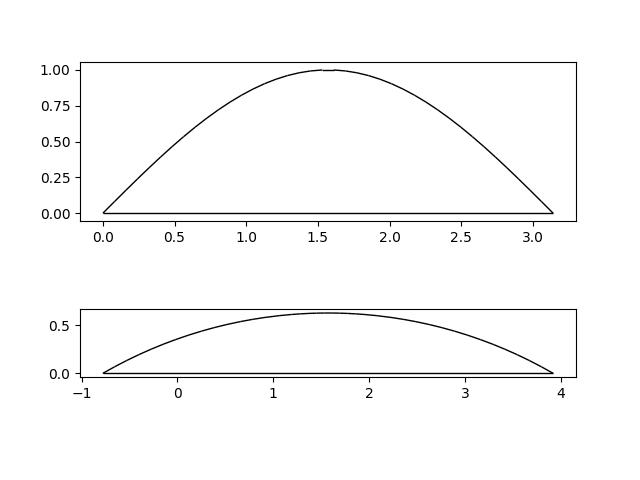
\includegraphics[width=0.6\linewidth]{figure/area1.png}
	\caption{液滴初试样貌为sinx在(0,$\pi$)}
	\label{fig:6}
\end{figure}
\begin{figure}[H]
	\centering
	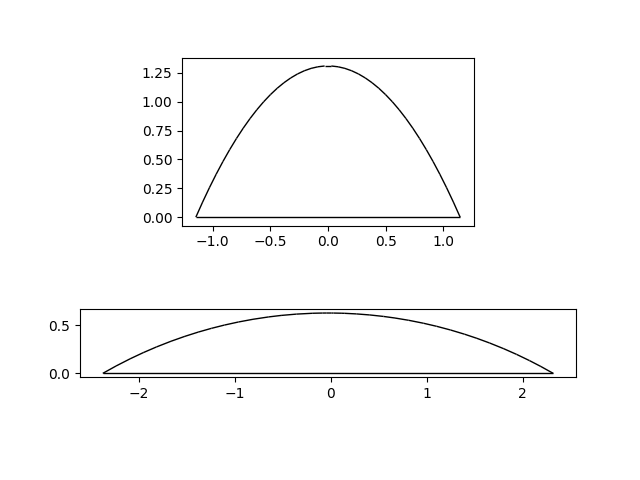
\includegraphics[width=0.6\linewidth]{figure/area2.png}
	\caption{液滴初试样貌为$x^2+\frac{3}{2}^\frac{2}{3}$在(-1,1)}
	\label{fig:7}
\end{figure}

\begin{center}
\renewcommand\arraystretch{3}
\begin{tabular}{|c|c|c|}
\hline 
\rule[-1ex]{0pt}{2.5ex} 模型初试样貌 & $\sin x$ & $x^2+\frac{3}{2}^{\frac{2}{3}}$ \\ 
\hline 
\rule[-1ex]{0pt}{2.5ex} 平衡时接触角角度 & 30.0 & 30.0 \\ 
\hline 
\rule[-1ex]{0pt}{2.5ex} 面积 & 1.99891 & 1.99868 \\ 
\hline 
\rule[-1ex]{0pt}{2.5ex} 结点个数 & 40 & 40 \\ 
\hline 
\rule[-1ex]{0pt}{2.5ex} 初始能量函数值 & 1.09917 & 1.65963 \\ 
\hline 
\rule[-1ex]{0pt}{2.5ex} 优化后能量函数值 & 0.85121 & 0.85120 \\ 
\hline 
\rule[-1ex]{0pt}{2.5ex} 迭代次数 & 1001 & 1001 \\ 
\hline 
\rule[-1ex]{0pt}{2.5ex} 初始接触角 & 44.96901 & 65.85403 \\ 
\hline 
\rule[-1ex]{0pt}{2.5ex} 优化后接触角 & 29.14710 & 29.04870 \\ 
\hline 
\end{tabular} 
\centerline{只改变初试样貌实验结果}
\end{center}

由图像和实验结果可以看出在控制面积、平衡时接触角一样的情况下,最终优化出来液滴样貌也是一样的,与预期结果吻合。

\newpage

\subsection{迭代次数}
这个数值实验是只改变迭代次数的情况下,看优化后的接触角是否能有效逼近平衡时的接触角。

\begin{center}
\renewcommand\arraystretch{2.2}
\begin{tabular}{|c|c|c|c|}
\hline 
\rule[-1ex]{0pt}{2.5ex} 模型初试样貌 & $-x^2+4$ & $-x^2+4$ & $-x^2+4$ \\ 
\hline 
\rule[-1ex]{0pt}{2.5ex} 平衡时接触角角度 & 30.0 & 30.0 & 30.0 \\ 
\hline 
\rule[-1ex]{0pt}{2.5ex} 结点个数 & 40 & 40 & 40 \\ 
\hline 
\rule[-1ex]{0pt}{2.5ex} 初始能量函数值 & 5.82776 & 5.82776 & 5.82776 \\ 
\hline 
\rule[-1ex]{0pt}{2.5ex} 初始接触角 & 75.60953 & 75.60953 & 75.60953 \\ 
\hline 
\rule[-1ex]{0pt}{2.5ex} 迭代次数 & 101 & 501 & 2501 \\ 
\hline 
\rule[-1ex]{0pt}{2.5ex} 优化后能量函数值 & 1.96902 & 1.96624 & 1.96571 \\ 
\hline 
\rule[-1ex]{0pt}{2.5ex} 优化后接触角 & 27.42186 & 28.86441 & 29.19596 \\ 
\hline 
\rule[-1ex]{0pt}{2.5ex} 接触角误差 & 2.57813 & 1.13558 & 0.80403 \\ 
\hline 
\end{tabular} 
\centerline{只改变迭代次数的实验结果}
\end{center}
\begin{figure}[H]
	\centering
	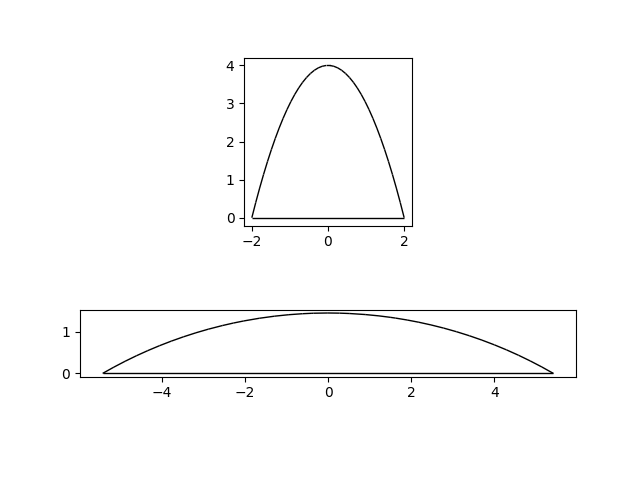
\includegraphics[width=0.7\linewidth]{figure/nit-p.png}
	\caption{迭代次数为1881优化前后图像}
	\label{fig:5}
\end{figure}
从实验结果可以看出随着迭代次数的增加,优化后的接触角在逼近平衡时的接触角。

\newpage

\subsection{网格步长}
这个数值实验是通过加密网格节点数来缩短网格的步长,使模型更加精细,看能否更好的逼近平衡时的接触角。

\begin{center}
\renewcommand\arraystretch{2.2}
\begin{tabular}{|c|c|c|c|}
\hline 
\rule[-1ex]{0pt}{2.5ex} 模型初试样貌 & 摆线 & 摆线 & 摆线 \\ 
\hline 
\rule[-1ex]{0pt}{2.5ex} 平衡时接触角角度 & 30.0 & 30.0 & 30.0 \\ 
\hline 
\rule[-1ex]{0pt}{2.5ex} 初始能量函数值 & 8.76097 & 8.76097 & 8.76097 \\ 
\hline 
\rule[-1ex]{0pt}{2.5ex} 初始接触角 & 86.92337 & 86.92337 & 86.92337 \\ 
\hline 
\rule[-1ex]{0pt}{2.5ex} 迭代次数 & 1001 & 1001 & 1001 \\ 
\hline
\rule[-1ex]{0pt}{2.5ex} 结点个数 & 40 & 80 & 160 \\ 
\hline  
\rule[-1ex]{0pt}{2.5ex} 优化后能量函数值 & 7.96958 & 7.96914 & 7.96711 \\ 
\hline 
\rule[-1ex]{0pt}{2.5ex} 优化后接触角 & 29.59781 & 29.93820 & 29.98273 \\ 
\hline 
\rule[-1ex]{0pt}{2.5ex} 接触角误差 & 0.4021 & 0.06179 & 0.01726 \\ 
\hline 
\end{tabular} 
\centerline{只改变网格步长的实验结果}
\end{center}
\begin{figure}[H]
	\centering
	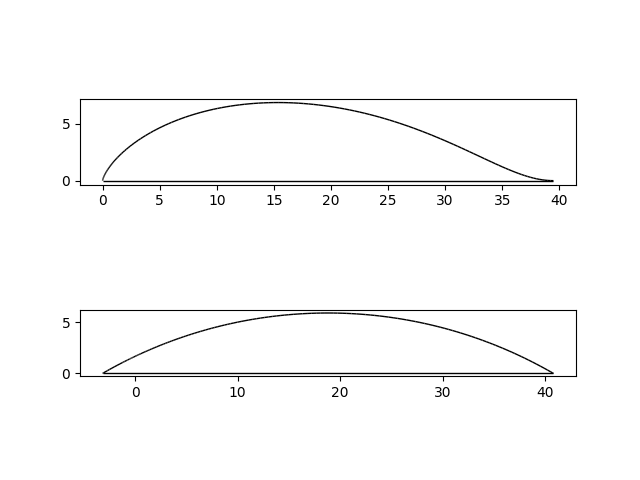
\includegraphics[width=0.7\linewidth]{figure/step-size-p.png}
	\caption{节点数为160时优化前后图像}
	\label{fig:1}
\end{figure}
从实验结果可以看出随着网格步长的加密,优化后的接触角在逼近平衡时的接触角。

\subsection{随机初试样貌}
为测试程序的适应性,我们生成三组随机的初试点,来看最终的结果
\begin{figure}[H]
	\centering
	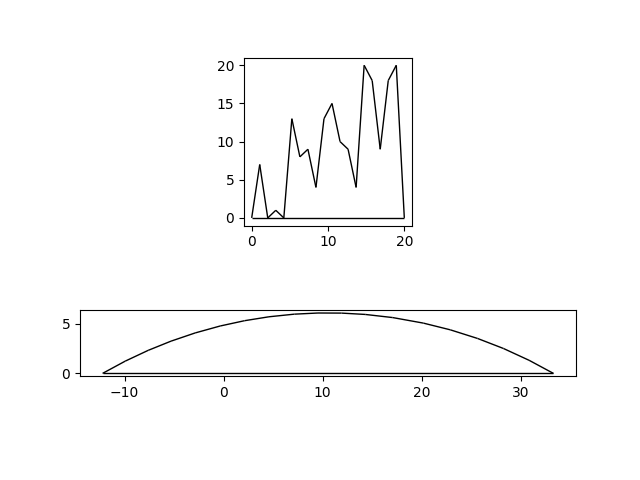
\includegraphics[width=0.7\linewidth]{figure/ran1.png}
	\caption{随机初始样貌1}
\end{figure}
\begin{figure}[H]
	\centering
	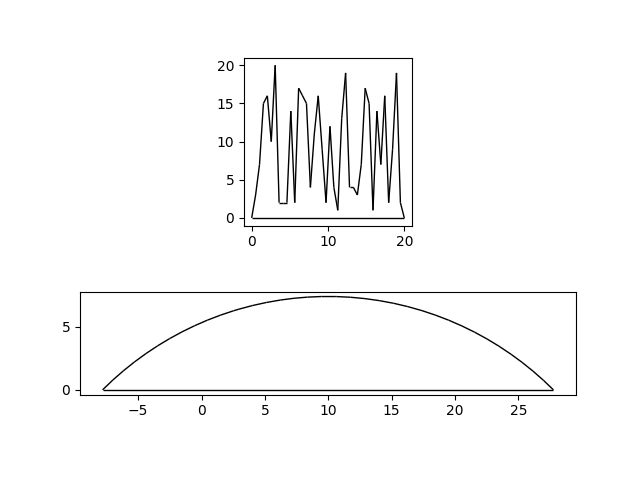
\includegraphics[width=0.7\linewidth]{figure/ran2.png}
	\caption{随机初始样貌2}
\end{figure}
\begin{figure}[H]
	\centering
	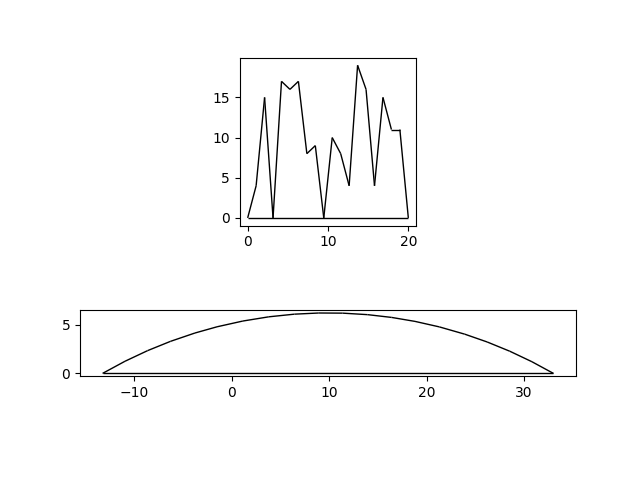
\includegraphics[width=0.7\linewidth]{figure/ran3.png}
	\caption{随机初始样貌3}
\end{figure}

\begin{center}
\renewcommand\arraystretch{2.2}
\begin{tabular}{|c|c|c|c|}
\hline 
\rule[-1ex]{0pt}{2.5ex} 模型初试样貌 & ran1 & ran2 & ran3 \\ 
\hline 
\rule[-1ex]{0pt}{2.5ex} 平衡时接触角角度 & 30.0 & 45.0 & 30.0 \\ 
\hline 
\rule[-1ex]{0pt}{2.5ex} 初始能量函数值 & 106.15208 & 280.54357 & 126.41692 \\ 
\hline 
\rule[-1ex]{0pt}{2.5ex} 初始接触角 & 81.44816 & 80.29961 & 75.25643 \\ 
\hline 
\rule[-1ex]{0pt}{2.5ex} 迭代次数 & 527 & 1677 & 300 \\ 
\hline
\rule[-1ex]{0pt}{2.5ex} 结点个数 & 20 & 40 & 20 \\ 
\hline  
\rule[-1ex]{0pt}{2.5ex} 优化后能量函数值 & 8.24649 & 14.3584 & 8.38353 \\ 
\hline 
\rule[-1ex]{0pt}{2.5ex} 优化后接触角 & 28.40358 & 43.74681 & 28.41881 \\ 
\hline 
\rule[-1ex]{0pt}{2.5ex} 接触角误差 &1.59641 & 1.25318 & 1.58118 \\ 
\hline 
\end{tabular} 
\centerline{随机实验结果}
\end{center}

上述三组随机的初试样貌程序都能有效的优化,该程序适应性由一定的保障
\newpage


\section{未来工作展望}
在本文的书写过程中,因为作者本身的知识有限和缺陷,也有一些工作尚未完成,系需要
之后的进一步探索。接下来研究价格主要从两方面展开:

1.本文只构建了液滴在二维情况下的数学模型,而三维才是现实中的实际情况,之后将
构建三维情况下的数学模型,有关三维问题需要用到曲面有限元等理论知识,还有待进一步的研究。

2.对于初试液滴样貌的逼近现在仅仅是二次的,之后会用高次曲线去逼近,并且也会尝试
选择更为有效的有限元算法来重新建立模型。

\newpage
\mbox{}
\newpage

\nocite{*}
\bibliographystyle{gbt7714-2005}
\bibliography{ref}
\newpage

\section*{附录}
模型代码实现主要用了numpy和feaply包,输入初始液滴样貌,实现可以返回梯度、面积和能量函数的功能。
\begin{python}
import numpy as np
from fealpy.mesh import IntervalMesh

class Model:
    def __init__(self, mesh, theta):
        self.mesh = mesh        
        self.theta = theta
        self.x0 = self.mesh.entity('node')  

    def __call__(self,x=None):
        mesh = self.mesh
        NN = mesh.number_of_nodes()
        cell = mesh.entity('cell')
        mesh.node = mesh.entity('node') if x is None else x.reshape(NN, 2)  #更新节点
        node = mesh.node
        theta = self.theta    
        gamma = np.cos(theta)
        h = mesh.entity_measure('cell')
        a = np.sum(h[:-1])    #液体气体接触面积
        b = np.sum(h[-1])     #液体固体接触面积
        val = a - gamma*b     #能量函数
        return val

    def gradient(self, x=None):
        mesh = self.mesh
        NN = mesh.number_of_nodes()
        cell = mesh.entity('cell')
        mesh.node = mesh.entity('node') if x is None else x.reshape(NN, 2)
        node = mesh.node
        theta = self.theta
        gamma = np.cos(theta)
        h = mesh.entity_measure('cell')
        v = mesh.cell_tangent()/h[:, np.newaxis]
        
        g = np.zeros((NN, 2), dtype=mesh.ftype)
        np.add.at(g, (cell[1:, 0], np.s_[:]), v[:-1])    #内部结点
        np.subtract.at(g, (cell[1:-1, 0], np.s_[:]), v[1:-1])
        
        g[0,0] = g[0,0] + gamma                          #端点
        g[-1]  = -v[0]
        g[-1,0] = g[-1,0] - gamma

        return g.reshape(-1)

    def volume(self, x=None):
        mesh = self.mesh
        NN = mesh.number_of_nodes()
        cell = mesh.entity('cell')
        mesh.node = mesh.entity('node') if x is None else x.reshape(NN, 2)
        node = mesh.node
        n = mesh.cell_normal()
        a = np.sum(n*node[cell[:, 0]])/2.0
        return a
\end{python}

\includepdf[pages={1}]{chart/check.pdf} 

\end{document}

